\documentclass[review]{elsarticle}\usepackage[]{graphicx}\usepackage[]{color}
%% maxwidth is the original width if it is less than linewidth
%% otherwise use linewidth (to make sure the graphics do not exceed the margin)
\makeatletter
\def\maxwidth{ %
  \ifdim\Gin@nat@width>\linewidth
    \linewidth
  \else
    \Gin@nat@width
  \fi
}
\makeatother

\definecolor{fgcolor}{rgb}{0.345, 0.345, 0.345}
\newcommand{\hlnum}[1]{\textcolor[rgb]{0.686,0.059,0.569}{#1}}%
\newcommand{\hlstr}[1]{\textcolor[rgb]{0.192,0.494,0.8}{#1}}%
\newcommand{\hlcom}[1]{\textcolor[rgb]{0.678,0.584,0.686}{\textit{#1}}}%
\newcommand{\hlopt}[1]{\textcolor[rgb]{0,0,0}{#1}}%
\newcommand{\hlstd}[1]{\textcolor[rgb]{0.345,0.345,0.345}{#1}}%
\newcommand{\hlkwa}[1]{\textcolor[rgb]{0.161,0.373,0.58}{\textbf{#1}}}%
\newcommand{\hlkwb}[1]{\textcolor[rgb]{0.69,0.353,0.396}{#1}}%
\newcommand{\hlkwc}[1]{\textcolor[rgb]{0.333,0.667,0.333}{#1}}%
\newcommand{\hlkwd}[1]{\textcolor[rgb]{0.737,0.353,0.396}{\textbf{#1}}}%
\let\hlipl\hlkwb

\usepackage{framed}
\makeatletter
\newenvironment{kframe}{%
 \def\at@end@of@kframe{}%
 \ifinner\ifhmode%
  \def\at@end@of@kframe{\end{minipage}}%
  \begin{minipage}{\columnwidth}%
 \fi\fi%
 \def\FrameCommand##1{\hskip\@totalleftmargin \hskip-\fboxsep
 \colorbox{shadecolor}{##1}\hskip-\fboxsep
     % There is no \\@totalrightmargin, so:
     \hskip-\linewidth \hskip-\@totalleftmargin \hskip\columnwidth}%
 \MakeFramed {\advance\hsize-\width
   \@totalleftmargin\z@ \linewidth\hsize
   \@setminipage}}%
 {\par\unskip\endMakeFramed%
 \at@end@of@kframe}
\makeatother

\definecolor{shadecolor}{rgb}{.97, .97, .97}
\definecolor{messagecolor}{rgb}{0, 0, 0}
\definecolor{warningcolor}{rgb}{1, 0, 1}
\definecolor{errorcolor}{rgb}{1, 0, 0}
\newenvironment{knitrout}{}{} % an empty environment to be redefined in TeX

\usepackage{alltt}
\usepackage[paperwidth=8.5in,paperheight=11in,top=1in,bottom=1in,left=1in,right=1in]{geometry}
\usepackage{setspace}
\usepackage[colorlinks=true,allcolors=Blue]{hyperref}
\usepackage{lineno}
\usepackage{cleveref}
\usepackage{acronym}
\usepackage{paralist}
\usepackage{bm}
\usepackage{fixltx2e}
% \usepackage[inline]{showlabels}

\journal{Ecological Modelling}

% biblio options
\bibliographystyle{elsarticle-harv}
\biboptions{authoryear}

% cleveref options
\crefname{table}{Table}{Tables}
\crefname{figure}{Fig.}{Figs.}
\renewcommand{\figurename}{Fig.}

%acronyms
\acrodef{chla}[chl-\textit{a}]{chlorophyll \textit{a}}
\acrodef{cgem}[CGEM]{Coastal General Ecosystem Model}
\acrodef{do}[O$_2$]{dissolved oxygen}
\acrodef{dom}[DOM]{dissolved organic matter}
\acrodef{gom}[GOM]{Gulf of Mexico}
\acrodef{lcs}[LCS]{Louisiana continental shelf}
\acrodef{marb}[MARB]{Mississippi-Atchafalaya River Basin}
\acrodef{pom}[POM]{particulate organic matter}
\acrodef{rmse}[\textit{RMSE}]{root mean squared error}
\acrodef{zerod}[0-D]{zero-dimensional}

%for supplemental figures/tables
\newcommand{\beginsupplement}{%
        \setcounter{table}{0}
        \renewcommand{\thetable}{S\arabic{table}}%
        \setcounter{figure}{0}
        \renewcommand{\thefigure}{S\arabic{figure}}%
     }

% invisible section anchor
\newcommand\invisiblesection[1]{%
  \refstepcounter{section}%
  \addcontentsline{toc}{section}{\protect\numberline{\thesection}#1}%
  \sectionmark{#1}}

% macro fix for multiple asterisks for corr author
\makeatletter
\def\@author#1{\g@addto@macro\elsauthors{\normalsize%
    \def\baselinestretch{1}%
    \upshape\authorsep#1\unskip\textsuperscript{%
      \ifx\@fnmark\@empty\else\unskip\sep\@fnmark\let\sep=,\fi
      \ifx\@corref\@empty\else\unskip\sep\@corref\let\sep=,\fi
      }%
    \def\authorsep{\unskip,\space}%
    \global\let\@fnmark\@empty
    \global\let\@corref\@empty  %% Added
    \global\let\sep\@empty}%
    \@eadauthor={#1}
}
\makeatother

% fix warning if acronyms are reset after abstract
\makeatletter
\renewcommand*\@verridelabel[1]{%
  \@bsphack
  \protected@write\@auxout{}{\string\undonewlabel{#1}}%
  \protected@write\@auxout{}{\string\undonewlabel{#1@cref}}%Added for cleverref
  \label{#1}%
  \@overriddenmessage rs{#1}%
  \@esphack
}%
\makeatother

\linespread{2}

%knitr options


% R dependencies


% get the version from git log


% get online bib file


\IfFileExists{upquote.sty}{\usepackage{upquote}}{}
\begin{document}
\large

\begin{frontmatter}

\title{Parameter sensitivity and identifiability for a biogeochemical model of hypoxia in the northern {G}ulf of {M}exico\tnoteref{mytitlenote}}
\tnotetext[mytitlenote]{Version: Tue Aug 15 18:37:33 2017 -0500, \href{https://github.com/fawda123/identifiability/commit/b9430cdc1b195b992ae6ea786f8e485723cf540c}{b9430cdc1b195b992ae6ea786f8e485723cf540c}\newline Acronyms: \acfi{chla}; \acfi{cgem}; \acfi{do}; \acfi{dom}; \acfi{gom}; \acfi{lcs}; \acfi{marb}; \acfi{pom}; \acfi{rmse}; \acfi{zerod}}

\date{}

\author{Marcus W. Beck\corref{mycorrespondingauthor}}
\address{USEPA National Health and Environmental Effects Research Laboratory, Gulf Ecology Division, 1 Sabine Island Drive, Gulf Breeze, FL 32561}
\cortext[mycorrespondingauthor]{Corresponding author}
\ead{beck.marcus@epa.gov}

\author{John C. Lehrter}
\address{University of South Alabama, Dauphin Island Sea Lab, Dauphin Island, AL 36528}
\ead{jlehrter@disl.org}

\author{Lisa L. Lowe}
\address{CSRA, Inc. supporting the USEPA, Research Triangle Park, NC 27709}
\ead{lowe.lisa@epa.gov}

\author{Brandon M. Jarvis}
\address{USEPA National Health and Environmental Effects Research Laboratory, Gulf Ecology Division, 1 Sabine Island Drive, Gulf Breeze, FL 32561}
\ead{jarvis.brandon@epa.gov}

% number of parameters evaluated, total and by category


\begin{abstract}
\noindent Local sensitivity analyses and identifiable parameter subsets were used to describe numerical constraints of a hypoxia model for bottom waters of the northern Gulf of Mexico.  The sensitivity of state variables differed considerably with parameter changes, although most variables were responsive to changes in parameters that influenced planktonic growth rates and less sensitive to physical or chemical parameters.  Variation in sensitivity had a direct correspondence with identifiability, such that only small subsets of the complete parameter set had unique effects on the model output. Selecting parameters by decreasing sensitivity demonstrated that only eight of 51 total parameters had a sufficiently unique effect on model output for accurate calibration.  As a result, parameter selection heuristics were used to identify parameters for model calibration that depended on combined effects on output, relative sensitivity of each parameter, and ecological categories for the biogeochemical equations. The calibrated \ac{zerod} unit of the hypoxia model had improved fit to the observed data if sensitive parameters were included in an identifiable subset.  Extension of results to a three-dimensional grid of the Gulf of Mexico showed that sensitive parameters for the \ac{zerod} model translated to non-trivial changes in the areal estimates of hypoxia.
\end{abstract}

\begin{keyword}
\ac{cgem}, \ac{gom}, Hypoxia, Identifiability, Sensitivity
\end{keyword}

\end{frontmatter}

% \linenumbers
\acresetall

\section{Introduction}

Hypoxia formation in bottom waters of coastal oceans occurs primarily from excess nutrient inputs from land-based sources \citep{Justic87,Diaz95,Howarth96}.  These events are detrimental to aquatic organisms and have significant negative effects on economic resources derived from coastal ecosystems \citep{Lipton03,Diaz11}.  An understanding of the biological, physical, and chemical processes that influence hypoxic areas is a critical concern for mitigating and preventing these negative impacts.  Numerical ecosystem models are important tools that synthesize knowledge of ecosystem processes that contribute to hypoxia formation and for predicting the effects of proposed management activities or future scenarios \citep{Scavia04,Hagy07,Camacho14a,Pauer16}.  Unlike statistical models with more generic structures, simulation and process-based models include explicit descriptions of relevant processes that are constrained by empirical or observational data relevant to the system of interest \citep[e.g.][]{Omlin01b,Eldridge10}.  These models are often coupled with hydrodynamic grids to provide spatially-explicit representations of patterns in three dimensions \citep{Warner05,Dortch07,Zhao10,Ganju16}. Combined hydrodynamic and bio-geo-chemical models have been developed specifically to describe hypoxic conditions on the \ac{lcs} in the northern \ac{gom} \citep{Fennel13,Obenour15,Pauer16,Lehrter17}.  This area drains a significant portion of the continental United States through the \ac{marb} and is the second largest hypoxic area in the world \citep{Rabalais02}.  Understanding processes that contribute to the frequency and duration of hypoxic events remains a critical research goal for the region.  

The development of a model represents a tradeoff between achieving predictive accuracy and a realistic representation of environmental processes. An ideal model is sufficiently generalizable across systems, provides results that are accurate given the inputs, and includes components that are valid descriptions of actual processes \citep{Levins66, Ganju16}. Given that these characteristics cannot be simultaneously achieved, models are developed that balance predictive accuracy with environmental realism, often favoring one at the expense of the other \citep{Morrison99,Ganju16}.  These challenges are analagous to the well-known bias-variance tradeoff in statistical models that balances the competing objectives of over- and under-fitting to an observed dataset. Process-based models are more commonly imbalanced between reality and theory, such that most are over-parameterized in an attempt to completely describe reality \citep{Denman03,Nossent12,Petrucci14}.  Quantitative limitations of over-parameterization are analagous to degrees of freedom in standard statistical models as free parameters cannot be numerically estimated when constrained to an observed dataset \citep{Kirchner06}.  More importantly, over-parameterization can limit use across systems outside of the data domain and impose uncertainty in model predictions as realistic values for every variable may not be known or inaccurately applied from existing studies \citep{Durand02,Refsgaard07,Wade08}.

Model fit can be evaluated relative to the effects of initial conditions or the observed data used for calibration, changes in parameter values, or variation in the structural components (i.e., observational, parameter, or structural uncertainty) \citep{Beck87}.  Evaluating effects of parameter changes is by far the most common and simplest approach.  Although sensitivity analyses should be integrated with model development, parameters are often evaluated post-hoc as a form of `damage control' for further calibration.  This approach is sometimes called inverse modelling where results from sensitivity analyses are used to guide calibration or fit of the developed model to observations (\citealt{Soetaert10}, or confronting models with data, \textit{sensu} \citealt{Hilborn97}).  Parameter sensitivity analysis combined with inverse modelling necessarily involves questions of parameter `identifiability'.  Redundancies in parameter effects lead to unidentifiable models where calibration is empirically impossible (i.e., standard algorithms will not converge) or parameter values may be non-unique leading to the right answer for the wrong reason \citep{Kirchner06}. Unidentifiable parameter sets have effects on model output that can be undone or compensated for by alteration of other parameters.  Identifiability issues are not foreign to hypoxia or eutrophication models  \citep{Omlin01,Estrada10,Mateus15}, although there is a clear need for greater integration of these concepts in practice \citep{Fasham06}.

This study describes a sensitivity and identifiability analysis of a \ac{zerod} unit of a larger spatial-temporal model of hypoxia dynamics on the \ac{lcs}.  The objectives were to provide a statistical approach that demonstrates numerical limitations of parameter sets for model calibration and provide a framework for selecting parameters within the identifiability constraints.  The specific goals were to \begin{inparaenum}[1\upshape)]
\item identify the parameters that have the greatest influence on state variables using local sensitivity analysis,
\item quantify the identifiability of subsets of the total parameter space based on sensitivity,
\item and provide a set of heuristics for choosing parameters based on sensitivity, identifiability, and parameter categories.
\end{inparaenum}
The \ac{zerod} model was calibrated with selected parameter subsets to demonstrate use of the selection heuristics to improve model fit.  Sensitive parameters for the \ac{zerod} model were also varied in the larger 3-dimensional model to demonstrate scalability of the results. In addition to \ac{do}, other state variables that were evaluated included ammonium, \ac{chla}, irradiance, nitrate, \ac{pom}, \ac{dom}, and phosphorus. In general, we provide empirical results to support the assumption that models are generally over-parameterized and only a finite and smaller subset of the complete parameter set can be optimized.

\section{Materials and Methods}

\subsection{Model description}

Hypoxic events, defined  as $<$2 mg L$^{-1}$ of \ac{do} ($<$ 64 mmol m$^{-3}$), occur seasonally in bottom waters in the northern \ac{gom}.  The hypoxic area averages 15,540 km$^2$ annually (1993-2015) with minimum concentrations observed from late spring to early fall.  Seasonal variation is strongly related to carbon and nutrient export from the \ac{marb} \citep{Lohrenz08,Bianchi10}, whereas hydrologic variation, currents, and wind patterns can affect vertical salinity gradients that contribute to hypoxia formation \citep{Wiseman97,Paerl98,Obenour15}. The \ac{cgem} was developed to describe hypoxia dynamics on the \ac{lcs} and includes elements from the Navy Coastal Ocean Model \citep{Martin00} for hydrodynamics and a biogeochemical model with multiple plankton groups, water-column metabolism, and sediment diagenesis \citep{Eldridge10}.  The hydrodynamic component of \ac{cgem} provides a spatially-explicit description of hypoxia using an orthogonal grid with an approximate horizontal resolution of 1.9 km$^2$ and twenty equally-spaced vertical sigma layers on the shelf.  The biogeochemical component includes equations for 36 state variables including six phytoplankton groups (with nitrogen and phosophorus quotas for each), two zooplankton groups, nitrate, ammonium, phosphate, dissolved inorganic carbon, oxygen, silica, and multiple variables for dissolved and particulate organic matter from different sources.

The core unit of \ac{cgem} is FishTank, a \ac{zerod} model that implements the biogeochemical equations in \citet{Eldridge10} and does not include any advection, mixing, or sediment diagenesis (\cref{fig:fishmod}). A full description of the model structure, equations, and parameters is described in appendices A-F in \citet{Lehrter17}. Although FishTank was developed for specific application in \ac{cgem}, it can easily be applied to other hydrodynamic grids. Results are based on time-dependent differential equations that describe energy flow between phytoplankton and zooplankton groups given nutrient uptake rates, organic matter inputs and losses, inherent optical properties, and temperature (\citealt{Penta08,Eldridge10}, see appendices in \citealt{Lehrter17}). A total of 108 equations are estimated at each time step to return values for each of the 36 state variables described by the model.  In addition to the initial conditions, 251 parameter values for each of the equations are also supplied at model execution. Values for each of the parameters were based on estimates from the literature, field or laboratory-based measurements, or expert knowledge in absence of the former.  As such, a sensitivity analysis of parameter values is warranted given that, for example, literature or field-based estimates may not apply under all scenarios or expert knowledge is not completely certain \citep{Refsgaard07}.

The sensitivity of state variables to perturbations of all relevant parameters for the 108 equations was estimated using a five minute timestep with daily output from January 1\textsuperscript{st} to December 31\textsuperscript{st}, 2006. Irrelevant parameters were removed for several reasons; parameters were not relevant for the \ac{zerod} model (i.e., hydrodynamic parameters), were considered physical constants, or had no effect given initial conditions.  Additionally, FishTank includes six phytoplankton and two zooplankton groups to add complexity in community structure and foodweb dynamics. To remove obvious redundancies, the sensitivity analyses were conducted using only one phytoplankton and one zooplankton group.  The final set that was evaluated included 51 parameters that were further grouped into one of six categories based on applicable biogeochemical components of the model: optics ($n = $ 4 parameters), organic matter (12), phytoplankton (22), temperature (2), and zooplankton (11) (\cref{tab:parmtab}).  A full description of the model parameters is available as an appendix in \citet{Lehrter17}.  

\subsection{Local sensitivity analysis}

A local sensitivity analysis was performed by evaluating the change in state variables following perturbation of each parameter from its original value \citep{Soetaert10,Camacho14b,RDCT17}. This approach is described as a First Order Variance Analysis that linearly propagates changes from model parameters to model predictions \citep{Camacho14b}. Parameters were individually perturbed by a 50\% increase of the original values (\cref{tab:parmtab}) and sensitivity $S$ was estimated for each time step $i$ given a change for parameter $j$ as:

\begin{equation} \label{sijeqn}
S_{ij} = \frac{\partial y_i}{\partial \Theta_j}\cdot\frac{w_{\Theta_j}}{w_{y_i}}
\end{equation}

\noindent where the estimate is based on the change in the predicted value for response variable $y$ divided by the change in the parameter $\Theta_j$ multiplied by the quotient of scaling factors $w$ for each.  The scaling factors, $w_{\Theta_j}$ for the parameter $\Theta_j$ and $w_{y_i}$ for response variable $y_i$, were set as the default value of the unperturbed parameter and the predicted value of $y_i$ after perturbation \citep{Soetaert10}.  Scaling makes the estimates unitless to compare model sensitivity to parameters and state variables that differ in relative magnitude.  Sensitivity values for all $j$ parameters were summarized as a single value across the time series from $i = 1$ to $n$ as $L1$:

\begin{equation} \label{l1}
L1 = \sum|S_{ij}|/n
\end{equation}

All parameters for each of the six equation categories (optics, organic matter, phytoplankton, temperature, and zooplankton) that had non-zero $L1$ were retained for identifiability analysis.  

\subsection{Identifiability and selecting parameter subsets}

The collinearity index $\gamma$ provides a measure of potential redundancies in the response of a state variable to changes in parameter values.  The index measures the linear dependence between sensitivity functions (i.e., $S_i$ for $j$ parameters) described above for parameter subsets and was estimated from the minimum eigenvector of the cross-product of a selected sensitivity matrix \citep{Brun01,Omlin01}:

\begin{equation} \label{gameq}
\gamma = \frac{1} {\sqrt{ \min \left(\rm{EV}[\mathit{\hat{S}}^\top \mathit{\hat{S}}]\right)}}
\end{equation}

\noindent where $\gamma$ ranges from one to infinity for perfectly identifiable (orthogonal) or unidentifiable (perfectly collinear) parameter sets.  The sensitivity functions were supplied as a matrix $\hat{S}$ with rows $i$ and columns $j$ (\cref{sijeqn}) that described deviations of predicted \ac{do} following perturbations of each parameter.  Thus, $\gamma$ can be estimated from results for any subset of parameter combinations. Sensitivity matrices were first normalized by dividing by the square root of the summed residuals \citep{Omlin01,Soetaert10}. Estimates of $\gamma$ greater than 10-15 suggest parameter sets are poorly identifiable \citep{Brun01,Omlin01}, meaning parameter values that maximize fit on a calibration dataset are inestimable by conventional optimization algorithms. An intuitive interpretation of $\gamma$ is provided by \citet{Brun01}, such that a change in a state variable caused by a change in one parameter can be offset by the fraction $1 - 1/\gamma$ by the remaining parameters.  That is, $\gamma = 10$ suggests the relative change in \ac{do} for an arbitrary parameter in the selected set can be compensated for by 90\% with changes in the other parameters. 

Parameter selection for model calibration must consider the competing objectives of increased goodness of fit with parameter inclusion and reduced identifiability as it relates to optimization.  An additional challenge is a large number of combinations of parameter sets, which complicates selection given sensitivity differences and desired ecological categories of each parameter (e.g., parameters for a group of related structural equations could be of interest).  \cref{fig:combnex} provides a simple graphic of the unique number of combinations that are possible for different subsets of `complete' parameter sets of different sizes (i.e., $n$ choose $k$ combinations, $n!/\left(k!\left(n-k\right)!\right)$).  The number of unique combinations increases with the total parameters in the set and is also maximized for moderate selections (e.g., selecting half the total).  For example, over 10$^{14}$ combinations are possible by selecting 25 parameters from a set of 50.

A set of heuristics was developed that addresses the tradeoff in model complexity and identifiability given the challenges described above \citep[see also][]{Wagener01}.  These rulesets were developed to select parameters with preference for those with high sensitivity and identifiability based on $\gamma < 15$ as an acceptable threshold for subsets (e.g., 93\% accountability between parameters).  Heurestics for parameter selection also recognized that parameter categories (i.e., optics, organic matter, phytoplankton, temperature, zooplankton) may have unequal preferences by users given desired application of the model.  For all selection heuristics, parameters were selected by decreasing sensitivity starting with the most sensitive until identifiability did not exceed $\gamma = 15$ where selections were \begin{inparaenum}[1\upshape)]
\item blocked within each of five parameter categories,
\item independent of parameter category,
\item or considering all categories equally.
\end{inparaenum}

\subsection{Model calibration and scalability}

Selected parameter subsets from the seven heuristics were used to calibrate the \ac{zerod} model.  This analysis demonstrated that different parameter sets can produce model output with differing goodness of fit and calibration effort given
\begin{inparaenum}[1\upshape)]
\item differences in variable sensitivity to parameters in each subset, 
\item differences in the parameters selected from different categories (heuristic difference), and 
\item differences in identifiability values.
\end{inparaenum}
Generally, this analysis was a proof of concept that the selection heuristics can lead to an `optimal' model by maximizing the balance between sensitivity and identifiability.  

Estimates of oxygen production from closed bottle experiments were used to calibrate the \ac{zerod} model.  Surface water was collected from a fixed location in Pensacola Bay, Florida () on September 25\textsuperscript{th}, 2013.  Water samples were placed into closed 100 mL glass bottles at the time of collection and transported back to the lab for treatments.  Concentrations of \ac{do} and nutrients (NH$_4^+$, NO$_2^-$, NO$_3^-$, PO$_4^{3-}$, and SiO$_3^{2-}$) were extracted from the samples within one hour of collection. Oxygen concentrations were established using Winkler reagents (Parsons et al. 1985) and titration using a MetrOhm Titrando with thiosulfate titrant calibrated against an iodate standard and electrochemical endpoint detection.  Ammonium was analyzed using a fluorometric method (Holmes et al. 1999); other nutrients were analyzed using either a Thermo Fisher Aquakem 200 discrete analyzer or an Astoria-Pacific continuous flow analyzer using standard colorimetric methods (APHA 2005).  

Oxygen production after an approximate 12 hour period was estimated within the bottles using three treatments: light, dark, and light plus nutrients.  All treatments were allowed to sit under ambient outdoor conditions in a water bath with continuous flow at the laboratory.  The dark treatments used opaque black bottles to ensure no exposure of ambient light to the samples.  The nutrient treatments were supplemented with an equal mix of 25 mmol m$^{-3}$ of ammonium and nitrate and 1.7 mmol m$^{-3}$, approximately two order of magnitude above ambient concentrations.  The exposure experiments began at 7am and were concluded at 7pm, after which the concentrations of \ac{do} in each bottle were measured.  Four replicates of each treatment were used. HOBO\textsuperscript{\textregistered} pendants were used to measure continous temperature and light for each treatment.  

Each parameter subset was calibrated to the ending \ac{do} concentration for each of the four replicates per treatment.   The intial values Parameter values were searched using the optim function in R that implemented the limited memory modification of the BFGS quasi-Newton method \citep{Byrd95,Nocedal06,RDCT17}.  This optimization scheme searches for values within the user-defined lower and upper bounds of each parameter.  We set the algorithm to search within an expected range chosen by the authors to best reflect...  While we recognize that `actual' parameter values could possibly extend beyond this range, constraining the values to the range tested herein was expected to produce output that was more interpretable within the context of the sensitivity functions defined above.  Moreover, precise limits on each parameter were less of a concern for the current analysis as our primary goal was to demonstrate differences in fit as a function of sensitivity and identifiability.  The optimal values for each parameter were identified based on convergence of the model results as a minimization of the \ac{rmse} between the observed and modelled data.    

As a final analysis, effects of parameter changes on the larger 3-dimensional model were evaluated to demonstrate that results from the \ac{zerod} FishTank model are scalable.  For simplicity, only the most sensitive parameter in each category was selected.  The \ac{cgem} model was run for one year using the default parameter conditions and by increasing each of the selected parameters by 50\%.  This produced six spatially-referenced time series (one default, five for each parameter change) from which changes in the daily hypoxic area (number of cells $<$ 64 mmol \ac{do}) were estimated.

\section{Results}

% for inline

 
\subsection{Local sensitivity analysis}

Local sensitivity analyses showed that \ac{do} was sensitive to perturbations in 38 of the 51 (75\% of total) parameters that were evaluated in FishTank (\cref{fig:sensalltile}, \cref{tab:dosens}). Within each parameter category, \ac{do} was sensitive to three parameters for optics (75\% of all optic parameters), eight for organic matter (67\%), 16 for phytoplankton (73\%), one for temperature (50\%), and 10 for zooplankton (91\%). Although \ac{do} had the greatest sensitivity to parameters in the zooplankton category (as percentage of total), the relative effects varied. Among all parameters, average sensitivity was $L1 = $ $9.2\times 10^{-3}$ with values ranging from $L1 = $ $8.34\times 10^{-8}$ for \textit{QminP} (phytoplankton) to $0.05$ for \textit{umax} (phytoplankton). Within categories (excluding temperature with one sensitive parameter), sensitivity ranged from $4.39\times 10^{-5}$ (\textit{astarOMA}) to $7.51\times 10^{-4}$ (\textit{astar490}) for optics, $4.17\times 10^{-4}$ (\textit{KNH4}) to $6.15\times 10^{-3}$ (\textit{KG1}) for organic matter, $8.34\times 10^{-8}$ (\textit{QminP}) to $0.05$ (\textit{umax}) for phytoplankton, and $3.69\times 10^{-5}$ (\textit{ZQp}) to $0.05$ (\textit{ZKa}) for zooplankton (\cref{tab:dosens}).  Average sensitivity values in each category were $L1 = $ $2.81\times 10^{-4}$ for optics, $2.17\times 10^{-3}$ for organic matter, $0.02$ for temperature, $0.01$ for phytoplankton, and $0.01$ for zooplankton.



Local sensitivity analyses for the additional state variables (ammonium, \ac{chla}, irradiance, nitrate, \ac{pom}, \ac{dom}, and phosphorus) had similar results as \ac{do} with some exceptions (\cref{fig:sensalltile,tab:nh4sens,tab:chlsens,tab:irrsens,tab:no3sens,tab:om1sens,tab:om2sens,tab:po4sens}).  All variables were sensitive to the same parameters as \ac{do} (38 of 51 evaluated), although average sensitivity differed between variables.  Average $L1$ ranged from $0.02$ for irradiance (\cref{tab:irrsens}) to $0.71$ for \ac{dom} (\cref{tab:om2sens}).  All average sensitivity values for the state variables were higher than the average for \ac{do} ($L1$ = $9.2\times 10^{-3}$).  For each variable, $L1$ ranged from $2.24\times 10^{-6}$ (\textit{QminP}) to $8.49$ (\textit{mA}) for ammonium (\cref{tab:nh4sens}), $1.38\times 10^{-6}$ (\textit{QminP}) to $13.94$ (\textit{mA}) for \ac{chla} (\cref{tab:chlsens}), $1.92\times 10^{-7}$ (\textit{QminP}) to $0.13$ (\textit{ZKa}) for irradiance (\cref{tab:irrsens}), $6.67\times 10^{-7}$ (\textit{QminP}) to $8.49$ (\textit{umax}) for nitrate (\cref{tab:no3sens}), $6.41\times 10^{-5}$ (\textit{KNH4}) to $7.22$ (\textit{mA}) for \ac{pom} (\cref{tab:om1sens}),  $7.41\times 10^{-5}$ (\textit{KNH4}) to $14.25$ (\textit{mA}) for \ac{dom} (\cref{tab:om2sens}), and $8.21\times 10^{-7}$ (\textit{QminP}) to $1.47$ (\textit{ZKa}) for phosphate (\cref{tab:po4sens}).  For the parameter categories, ammonium was most sensitive to phytoplankton parameters (average $L1$ = $0.8$ across all parameters in the category), \ac{chla} to phytoplankton ($L1$ = $1.14$), irradiance to zooplankton ($L1$ = $0.03$), nitrate to zooplankton ($L1$ = $1.06$), \ac{pom} to temperature ($L1$ = $0.86$), \ac{dom} to temperature ($L1$ = $1.48$), and phosphate to zooplankton ($L1$ = $0.31$).  Finally, average sensitivity between parameter categories independent of the state variables ranged from $8.38\times 10^{-3}$ for optics (average $L1$ across all variables) to $0.62$ for phytoplankton. 

\subsection{Identifiability of parameter subsets and selection rules}



The identifiability analyses suggested that many parameter subsets exceeded the thresholds of $\gamma = 10, 15$.  Parameter identifiability for \ac{do} decreased (increasing $\gamma$) at different rates with increasing size of parameter subsets depending on the parameter category or the number of top parameters that were selected (\cref{fig:identplo}). By category, identifiability was lowest for all combinations of parameter subsets in the phytoplankton ($60$\% of subsets less than $\gamma = 15$, $43$\% less than $\gamma = 10$) and zooplankton categories ($53.1$\% less than $\gamma = 15$, $40$\% less than $\gamma = 10$), whereas all combinations were identifiable for optics ($100$\% less than $\gamma = 15, 10$) and a majority identifiable for organic matter ($91.9$\% less than $\gamma = 15$, $76.5$\% less than $\gamma = 10$). Identifiability for parameters in the temperature category was not evaluated because \ac{do} was sensitive to only one parameter (i.e., $\gamma = 1$). Parameter combinations for choosing from the top, top two, top three, and top four parameters in each category together had decreasing identifiability with the increasing size of the selection pool (e.g., top one versus top four parameters, \cref{fig:identplo}).  The percentage of parameter subsets that were below the acceptable thresholds for identifiability was $100$\% less than $\gamma = 15, 10$ for the top parameter in each category, $90.6$\% and $80.7$\% for the top two, $80.7$\% and $70.9$\% for the top three, and $55.8$\% and $45.7$\% for the top four.  Results for the remaining state variables had similar patterns in identifiability with increasing size of parameter subsets and selection categories, although differences in identifiability between state variables was observed (\cref{fig:identploall}).  Most notably, nitrate was consistently the least identifiable variable (highest overall $\gamma$), whereas \ac{do} was most identifiable.



An evaluation of the effects of individual parameters on $\gamma$ suggested that some parameters had disproportionate effects on identifiability.  Based on $\gamma = 15$, \cref{fig:identplo} suggests that most parameter sets for organic matter were identifiable, regardless of how many parameters were selected (i.e., two through eight).  However, some subsets were not identifiable such that identification of one or more redundant parameters that are inflating $\gamma$ values could provide useful information.  \Cref{fig:exclex} shows an alternative view of identifiability of \ac{do} with exclusion and inclusion of individual parameters in different sets for the organic matter category.  As before, collinearity increases with more parameters in a subset, although the increase varies depending on which parameter was included or excluded from the set.  For example, inclusion of \textit{KNO3} in a parameter set almost always inflated $\gamma$.  All parameter subsets that did not include \textit{KNO3} were well below $\gamma = 15$, suggesting that exclusion of this parameter improves identifiability.  Interestingly, the inclusion of some parameters caused a reduction in $\gamma$, which contradicts the general rule that more parameters caused reduced identifiablity.  For example, parameter sets that included \textit{KGcdom} generally had lower $\gamma$ values relative to those that excluded the parameter.


Results for each of the three selection heuristics (blocked by parameter category, independent of category, all categories equally) applied to each state variable differed in the number of selected parameters and distribution of parameters within each category (\cref{tab:heurist1,tab:heurist2,tab:heurist3}).  In general, a corresponendence was observed between the number of parameters that were selected given the threhold of $\gamma = 15$ and relative identifiability between the state variables.  As noted above, nitrate was the least identifiable variable (\cref{fig:identploall}), whereas other variables (e.g., \ac{do}, irradiance) were more identifiable.  The constraints on identifiability between variables were demonstrated with the selection heuristics.  For example, heuristics for nitrate typically selected only one or two parameters that met the criteria as compared to more identifiable variables that included several parameters. Overall, the first selection heuristic demonstrated that the number of parameters chosen by parameter category differed independently of the state variables (\cref{tab:heurist1}). The number of selected parameters averaged across state variables in decreasing order was 4.25 parameters from the phytoplankton category, 3.5 from organic matter, 2.75 from optics, and 2.38 from zooplankton. The second and third selection heuristics (\cref{tab:heurist2,tab:heurist3}) were similar, although more parameters were generally selected for the third heuristic given equal importance between categories.

\subsection{Model calibration and scalability}



Calibration of parameter values for each of the seven selection heuristics (\cref{tab:heurist1,tab:heurist2,tab:heurist3})  produced model output that varied in goodness of fit and computational effort required to identify optimal values (\cref{tab:calib}).  As expected, the number of required iterations of the optimization algorithm to minimize \ac{rmse} of observed \ac{do} and model output varied in proportion to the number of parameters in a subset.  For example, only three iterations were required to optimize the single parameter selected for the temperature category, whereas 289 iterations were required for the eight parameters selected independent of category.  No association was observed between collinearity ($\gamma$) and number of iterations or calibration.  Of the seven parameter subsets, selection independent of parameter category and equally within each category produced the largest reduction in \ac{rmse} values from the default output (starting \ac{rmse} $35.33$ mmol O$_2$ m$^{-3}$, reduction to $35.29$, $35.32$, respectively), whereas the optimal values for parameters in the Optics category had the smallest reduction ($35.33$).  Lower \ac{rmse} was associated with higher average sensitivity of a parameter subset.  Parameters selected only in the optics category had the highest \ac{rmse} and lowest average L1 ($2.81\times 10^{-4}$, three parameters), whereas parameters selected independent of category had the lowest \ac{rmse} and highest average L1 ($0.03$, eight parameters, \cref{tab:calib}). 



The estimated areal extent of bottom-water hypoxia using default parameter values for the 3-dimensional model peaked on August, 28\textsuperscript{th} at $1.19\times 10^{4}$ km$^2$ (\cref{fig:areachg}a, August mean area 8988 $\pm$ 551 km$^2$, \cref{fig:areachg}b). Increases in the top sensitive parameters for \ac{do} in each category (\cref{tab:dosens}) increased the estimated areal extent of hypoxia (Figs. \ref{fig:areachg}c, \ref{fig:areachg}e), with the exception of the parameter for optimum temperature of growth (\textit{Tref(nospA+nospZ)$_{p1}$}), which caused a decrease (mean difference from July default area -1070 $\pm$ 1161 km$^2$, \cref{fig:areachg}d).  The largest increase in area was caused by an increase in the maximum growth rate of phytoplankton (\textit{umax}), with the greatest increase occurring in July (monthly mean increase of 4109 $\pm$ 1085 km$^2$, \cref{fig:areachg}d).  Overall, changes in hypoxia extent were largest for parameters with large sensitivity values (i.e., L1 = $0.05$ for \textit{ZKa}, L1 = $0.05$ for \textit{umax}).

\section{Discussion}

State variables were most sensitive to phytoplankton and zooplankton parameters, particularly the maximum growth rates (\textit{umax} for phytoplankton, \textit{Zumax} for zooplankton), mortality coefficient for phytoplankton (\textit{mA}), and the zooplankton half saturation coefficent for grazing (\textit{ZKa}). An increase in the growth rate of primary producers can increase oxygen concentration through photosynthetic processes, although increased production of organic matter is balanced with respiration and bacterial decomposition that reduce \ac{do} in the water column.  Similarly, increases in zooplankton abundance with increased growth rates can reduce phytoplankton biomass through grazing, which is expected to further deplete pools of organic matter from algal sources.  Most variables were also sensitive to variation in the half-saturation grazing coefficient which moderates nutrient concentrations that support half the maximum grazing rate. Although the tradeoff between abundance, grazing, and decomposition is complex, the sensitivity of model state variables to parameters that directly control the abundance of primary producers is in agreement with empirical observations of factors that influence hypoxia dynamics on the \ac{lcs} \citep{Fahnenstiel95,Roelke00,Eldridge10}. The sensitivity of the model output to variation in other parameters that relate to physical and chemical properties of the system was of secondary importance.  That is, state variables were sensitive to changes in light and temperature parameters, although to a lesser extent than biological parameters.  As such, the differing sensitivities of state variables to parameters in each of the categories was not unexpected given ecological relationships that are well understood and described by the model.    

A general conclusion from the identifiability analyses is that only limited subsets of parameters were identifiable within the constraints of local sensitivity analyses. These results support previous studies that have suggested similarly small subsets of parameters can be identified using traditional calibration schemes \citep[e.g.,][]{Wheater86,Ye97,Omlin01}.  In addition to \ac{cgem}, these conclusions have relevance for other biogeochemical models that include numerous parameters and structural equations to characterize processes in the model domain.  A general conclusion is that less complex models are potentially beneficial given that only a small subset of parameters is identifiable and that ecosystem processes may in fact be sufficiently characterized with few parameters \citep{Ye97}.  Conversely, others have argued that model complexity is not in itself a disadvantage when parsimony is not the only determinant of model structure \citep{Reichert97}. Over-parameterization can be useful if processes have importance that were not evaluated during model identification.  Single objective functions that maximize model fit with identifiable parameters may also provide an incomplete characterization of model worth, which has prompted the development of probability-based models of hypoxia that explicitly include uncertainty in model components \citep[e.g.][]{Obenour15}.  Our results demonstrated that approximately 75\% of the evaluated parameters had an effect on the eight state variables, whereas \ac{cgem} includes a total of 36 variables and multiple plankton groups, not all of which have immediate concern for understanding hypoxia. The redundancies identified with the sensitivity analyses are challenging only if the primary interest is, for example, \ac{do} dynamics.  Moreover, the proposed selection heuristics provide flexibility for choosing different parameters with the assumption that those chosen depend on the research or management question. 

Results from the identifiability analyses provided additional insight into the interactions of parameters in large biogeochemical models.  First, identifiability of parameter subsets was not related to the sensitivity of individual variables. As noted above, an identifiable parameter is one that has a unique effect on model predictions that cannot be compensated for or undone by changing other parameters. The magnitude of the effect of a parameter has no bearing on identifiability, which further complicates the selection of parameters for calibration.  Although identifiability is the primary limiting factor in choosing a set, the relative sensitivities are more important for the decision to include or exclude individual parameters.  For example, \cref{tab:calib,fig:areachg} demonstrated that parameter sets with sensitive parameters had improved model fit and that these parameters had affects that translated to the larger model. Our analysis addressed this challenge by presenting multiple selection criteria for identifiable parameter sets that prioritized the most sensitive parameters during the selection process.  Similarly, identifiability was not always related to the number of parameters in a set. Although the general trend was decreasing identifiability with more parameters, the unique effects of including an individual parameter with an existing set often reduced the $\gamma$ estimate. For example, \cref{fig:exclex} showed that including \textit{KGcdom}, \textit{KO2}, or \textit{nitmax} in parameter sets more often reduced $\gamma$ relative to sets that excluded the parameters.  The selection criteria proposed above can facilitate parameter selection and also provide diagnostic tools to identify parameters with disproportionate effects on $\gamma$.

\subsection{Recommendations and conclusions}

Our results demonstrated that small parameter subsets relative to all sensitive parameters were within the identifiability thresholds described in the literature.  The identifiable parameter subsets varied considerably between state variables and the method for parameter selection.  Use of identifiable parameter subsets with sensitive parameters improved model fit and results for the smaller model were scalable to the 3-dimensional model.  However, an evaluation of sensitivity and identifiability of relevant parameter sets is a preliminary and simplistic approach to improving model predictions.  We have provided a general approach to select parameter subsets for further model development depending on the ecological context (i.e., selection by parameter category, selection for specific state variables). Thus, the results described above have relevance for model refinement with the specific goal of better understanding ecological dynamics that moderate hypoxia on the northern \ac{gom}.  The general principles of sensitivity and parameter identifiability have broad applicability beyond this context and we argue that such methods should be more universally applied as an initial approach to quantify numerical constraints of biogeochemical models.  

The effects of structural or observational uncertainty could be evaluated as an extension of the analyses presented above. For example, the sensitivity of \ac{do} to variation in the half-saturation constants for phytoplankton (the concentration supporting half the maximum uptake rate of nutrients) could vary given the initial nutrient concentrations \citep{Eppley69}. Further, changes in the ratio between nitrogen and phosphorus could affect the sensitivity of state variables to parameter changes depending on the limiting nutrient.  A more challenging analysis is an evaluation of the effects of structural components on model output, which requires exclusion or inclusion of explicit biogeochemical equations. The FishTank model includes several `switches' that allow users to change the governing equations that estimate state variables, such as switches that `turn on' different structural equations for light attenuation in the water column.  This design is uncommon in biogeochemical models and could be leveraged for an evaluation of structural uncertainty. As such, our analysis of parameter sensitivity and identifiabilty could be combined with an evaluation of observational and structural uncertainty for a more complete characterization of the model, having implications for understanding drivers of hypoxia in coastal waters.  

\section*{Acknowledgments}

We thank the research staff of the USEPA Gulf Ecology Division, Environmental Modeling and Visualization Laboratory, and Naval Research Laboratory for their efforts developing the hydrodynamic and biogeochemical components of \ac{cgem}. We thank James Pauer, Yonghsan Wan, and Susan Elizabeth George for providing helpful comments on an earlier draft.

\section*{Role of Funding Sources}

This study was funded, reviewed, and approved for publication by the US EPA, National Health and Environmental Effects Research Laboratory.  However, the views expressed in this paper are those of the authors and do not necessarily reflect the views or policies of the US EPA. 

\clearpage

% \bibliography{refs}
\bibliography{refsshr}
\clearpage

%%%%%%
% tables

\invisiblesection{Tables}

% parameter info
%latex.default(totab, file = "", rowlabel = "Description", caption = cap.val,     caption.loc = "top", rowname = Description, rgroup = unique(cats),     n.rgroup = as.numeric(table(cats)), size = tabsize, label = paste0("tab:",         tablab), insert.bottom = foot.val)%
\begin{table}[!tbp]
{\tiny
\caption{FishTank parameters evaluated for sensitivity and identifiability. Sensitivitity analyses were based on a 50\% increase (Value $\cdot$ 1.5) from the initial value of each parameter. Dashed units are dimensionless. Parameters are grouped by categories as optics, temperature, phytoplankton, zooplankton, and organic matter.  A full description of the model structure, equations, and parameters is described in \citet{Lehrter17}.\label{tab:parmtab}} 
\begin{center}
\begin{tabular}{lllll}
\hline\hline
\multicolumn{1}{l}{Description}&\multicolumn{1}{c}{Parameter}&\multicolumn{1}{c}{Units}&\multicolumn{1}{c}{Value}&\multicolumn{1}{c}{Value $\cdot$ 1.5}\tabularnewline
\hline
{\bfseries Optics}&&&&\tabularnewline
~~Chla specific absorption at 490 nm&\textit{astar490}&m$^{-1}$ (mg Chla m$^{-3}$)$^{-1}$&$0.04$&$0.06$\tabularnewline
~~OMA specific absorption at 490 nm&\textit{astarOMA}&m$^{-1}$ (mg OMA m$^{-3}$)$^{-1}$&$0.1$&$0.15$\tabularnewline
~~OMZ specific absorption at 490 nm&\textit{astarOMZ}&m$^{-1}$ (mg OMZ m$^{-3}$)$^{-1}$&$0.1$&$0.15$\tabularnewline
~~sinking rate&\textit{sink CDOM}&m d$^{-1}$&$0$&$0$\tabularnewline
\hline
{\bfseries Temperature}&&&&\tabularnewline
~~Optimum temperature for growth&\textit{Tref(nospA+nospZ)$_{p1}$}&C&$22$&$33$\tabularnewline
~~Optimum temperature for growth&\textit{Tref(nospA+nospZ)$_{p1}$}&C&$22$&$33$\tabularnewline
\hline
{\bfseries Phytoplankton}&&&&\tabularnewline
~~initial slope of photosynthesis v irradiance&\textit{alpha}&10$^{-16}$ cm$^2$ s quanta$^{-1}$ d$^{-1}$&$8.42\times 10^{-17}$&$1.26\times 10^{-16}$\tabularnewline
~~coefficient for non-limiting nutrient&\textit{aN}&-&$1$&$1.5$\tabularnewline
~~phytoplankton threshold for grazing&\textit{Athresh}&10$^7$ cells m$^{-3}$&$1.72\times 10^{8}$&$2.58\times 10^{8}$\tabularnewline
~~edibility vector for Z1&\textit{ediblevector(Z1)}&-&$0.25$&$0.38$\tabularnewline
~~edibility vector for Z2&\textit{ediblevector(Z2)}&-&$0.25$&$0.38$\tabularnewline
~~half-saturation constant for N&\textit{Kn}&mmol m$^{-3}$&$4.51$&$6.76$\tabularnewline
~~half-saturation constant for P&\textit{Kp}&mmol m$^{-3}$&$2.86$&$4.29$\tabularnewline
~~Qn constant for Flynn growth model&\textit{KQn}&-&$5$&$7.5$\tabularnewline
~~Qp constant for Flynn growth model&\textit{KQp}&-&$0.2$&$0.3$\tabularnewline
~~half-saturation constant for Si uptake&\textit{Ksi}&mmol m$^{-3}$&$4.51$&$6.76$\tabularnewline
~~mortality coefficient&\textit{mA}&d$^{-1}$&$0.1$&$0.15$\tabularnewline
~~phytoplankton carbon/cell&\textit{Qc}&10$^{-7}$ mmol C cell$^{-1}$&$1.35\times 10^{-6}$&$2.03\times 10^{-6}$\tabularnewline
~~minimum N cell-quota&\textit{QminN}&10$^{-9}$ mmol N cell$^{-1}$&$6.08\times 10^{-9}$&$9.12\times 10^{-9}$\tabularnewline
~~minimum P cell-quota&\textit{QminP}&10$^{-9}$ mmol P cell$^{-1}$&$6.19\times 10^{-10}$&$9.29\times 10^{-10}$\tabularnewline
~~phytoplankton basal respiration coefficient&\textit{respb}&d$^{-1}$&$0.02$&$0.03$\tabularnewline
~~phytoplankton growth respiration coefficient&\textit{respg}&-&$0.1$&$0.15$\tabularnewline
~~sinking rate of phytoplankton cells&\textit{sink A}&m d$^{-1}$&$1.49$&$2.23$\tabularnewline
~~maximum growth rate&\textit{umax}&d$^{-1}$&$0.41$&$0.62$\tabularnewline
~~N-uptake rate measured at umax&\textit{vmaxN}&10$^{-8}$ mmol cell$^{-1}$ d$^{-1}$&$4.1\times 10^{-8}$&$6.15\times 10^{-8}$\tabularnewline
~~P-uptake rate measured at umax&\textit{vmaxP}&10$^{-8}$ mmol cell$^{-1}$ d$^{-1}$&$2.68\times 10^{-8}$&$4.02\times 10^{-8}$\tabularnewline
~~Si-uptake rate measured at umax&\textit{vmaxSi}&10$^{-8}$ mmol cell$^{-1}$ d$^{-1}$&$4.1\times 10^{-8}$&$6.15\times 10^{-8}$\tabularnewline
~~phytoplankton volume/cell&\textit{volcell}&$\mu$m$^3$&$3.37\times 10^{4}$&$5.05\times 10^{4}$\tabularnewline
\hline
{\bfseries Zooplankton}&&&&\tabularnewline
~~assimilation efficiency as a fraction of ingestion&\textit{Zeffic}&-&$0.4$&$0.6$\tabularnewline
~~half saturation coefficient for grazing&\textit{ZKa}&$\mu$m$^3$ m$^{-3}$&$1.12\times 10^{12}$&$1.68\times 10^{12}$\tabularnewline
~~quadratic mortality constant&\textit{Zm}&m$^6$ ind$^{-2}$ d$^{-1}$&$7.2\times 10^{-4}$&$0$\tabularnewline
~~zooplankton carbon/individual&\textit{ZQc}&mmol C ind$^{-1}$&$3.13\times 10^{-4}$&$4.7\times 10^{-4}$\tabularnewline
~~zooplankton nitrogen/individual&\textit{ZQn}&mmol N ind$^{-1}$&$6.95\times 10^{-5}$&$1.04\times 10^{-4}$\tabularnewline
~~zooplankton phosphorus/individual&\textit{ZQp}&mmol P ind$^{-1}$&$3.77\times 10^{-6}$&$5.66\times 10^{-6}$\tabularnewline
~~zooplankton biomass-dependent respiration factor&\textit{Zrespb}&d$^{-1}$&$0.1$&$0.15$\tabularnewline
~~zooplankton growth-dependent respiration factor&\textit{Zrespg}&-&$0.2$&$0.3$\tabularnewline
~~proportion of phytoplankton lost to sloppy feeding&\textit{Zslop}&-&$0.25$&$0.38$\tabularnewline
~~maximum growth rate of zooplankton&\textit{Zumax}&$\mu$m$^3$ ind$^{-1}$ d$^{-1}$&$9.45\times 10^{7}$&$1.42\times 10^{8}$\tabularnewline
~~zooplankton volume/individual&\textit{Zvolcell}&$\mu$m$^3$ ind$^{-1}$&$2.98\times 10^{7}$&$4.47\times 10^{7}$\tabularnewline
\hline
{\bfseries Organic Matter}&&&&\tabularnewline
~~turnover rate for OM1A and OM1Z&\textit{KG1}&y$^{-1}$&$50$&$75$\tabularnewline
~~turnover rate for OM2A and OM2Z&\textit{KG2}&y$^{-1}$&$50$&$75$\tabularnewline
~~decay rate of CDOM&\textit{KGcdom}&d$^{-1}$&$0.01$&$0.02$\tabularnewline
~~NH4 rate constant for nitrification&\textit{KNH4}&mmol m$^{-3}$&$1$&$1.5$\tabularnewline
~~half-saturation concentration for denitrification&\textit{KNO3}&mmol m$^{-3}$&$10$&$15$\tabularnewline
~~half-saturation concentration for O2 utilization&\textit{KO2}&mmol m$^{-3}$&$10$&$15$\tabularnewline
~~O2 concentration that inhibits denitrification&\textit{KstarO2}&mmol m$^{-3}$&$10$&$15$\tabularnewline
~~maximum rate of nitrification per day&\textit{nitmax}&mmol m$^{-3}$ d$^{-1}$&$0.52$&$0.78$\tabularnewline
~~phytoplankton sinking rate&\textit{sink OM1\_A}&m d$^{-1}$&$10$&$15$\tabularnewline
~~zooplankton sinking rate&\textit{sink OM1\_Z}&m d$^{-1}$&$10$&$15$\tabularnewline
~~phytoplankton sinking rate&\textit{sink OM2\_A}&m d$^{-1}$&$0$&$0$\tabularnewline
~~zooplankton sinking rate&\textit{sink OM2\_Z}&m d$^{-1}$&$0$&$0$\tabularnewline
\hline
\end{tabular}\end{center}}
\end{table}


% do sensitivity all categories
%latex.default(totab, file = "", rowlabel = "Description", caption = cap.val,     caption.loc = "top", rowname = Description, rgroup = unique(cats),     n.rgroup = as.numeric(table(cats)), size = tabsize, label = paste0("tab:",         tablab), insert.bottom = foot.val)%
\begin{table}[!tbp]
{\footnotesize
\caption{Sensitivity of \ac{do} to perturbations of individual parameters.  Sensitivities are based on a 50\% increase from the initial parameter value, where $L1$ summarizes differences in model output (see \cref{l1}).  Parameters that did not affect \ac{do} are not shown.  Parameters are grouped by categories as optics, temperature, phytoplankton, zooplankton, and organic matter.\label{tab:dosens}} 
\begin{center}
\begin{tabular}{lll}
\hline\hline
\multicolumn{1}{l}{Description}&\multicolumn{1}{c}{Parameter}&\multicolumn{1}{c}{L1}\tabularnewline
\hline
{\bfseries Optics}&&\tabularnewline
~~Chla specific absorption at 490 nm&\textit{astar490}&$7.51\times 10^{-4}$\tabularnewline
~~OMZ specific absorption at 490 nm&\textit{astarOMZ}&$4.92\times 10^{-5}$\tabularnewline
~~OMA specific absorption at 490 nm&\textit{astarOMA}&$4.39\times 10^{-5}$\tabularnewline
\hline
{\bfseries Organic Matter}&&\tabularnewline
~~turnover rate for OM1A and OM1Z&\textit{KG1}&$6.15\times 10^{-3}$\tabularnewline
~~turnover rate for OM2A and OM2Z&\textit{KG2}&$3.14\times 10^{-3}$\tabularnewline
~~O2 concentration that inhibits denitrification&\textit{KstarO2}&$3.04\times 10^{-3}$\tabularnewline
~~decay rate of CDOM&\textit{KGcdom}&$2.98\times 10^{-3}$\tabularnewline
~~half-saturation concentration for O2 utilization&\textit{KO2}&$5.85\times 10^{-4}$\tabularnewline
~~half-saturation concentration for denitrification&\textit{KNO3}&$5.8\times 10^{-4}$\tabularnewline
~~maximum rate of nitrification per day&\textit{nitmax}&$4.99\times 10^{-4}$\tabularnewline
~~NH4 rate constant for nitrification&\textit{KNH4}&$4.17\times 10^{-4}$\tabularnewline
\hline
{\bfseries Phytoplankton}&&\tabularnewline
~~maximum growth rate&\textit{umax}&$0.05$\tabularnewline
~~mortality coefficient&\textit{mA}&$0.02$\tabularnewline
~~initial slope of photosynthesis v irradiance&\textit{alpha}&$0.02$\tabularnewline
~~edibility vector for Z1&\textit{ediblevector(Z1)}&$0.02$\tabularnewline
~~phytoplankton carbon/cell&\textit{Qc}&$0.01$\tabularnewline
~~phytoplankton growth respiration coefficient&\textit{respg}&$8.36\times 10^{-3}$\tabularnewline
~~N-uptake rate measured at umax&\textit{vmaxN}&$8.12\times 10^{-3}$\tabularnewline
~~phytoplankton basal respiration coefficient&\textit{respb}&$6.94\times 10^{-3}$\tabularnewline
~~phytoplankton threshold for grazing&\textit{Athresh}&$4.57\times 10^{-3}$\tabularnewline
~~minimum N cell-quota&\textit{QminN}&$4.32\times 10^{-3}$\tabularnewline
~~P-uptake rate measured at umax&\textit{vmaxP}&$4.27\times 10^{-3}$\tabularnewline
~~coefficient for non-limiting nutrient&\textit{aN}&$4.23\times 10^{-3}$\tabularnewline
~~phytoplankton volume/cell&\textit{volcell}&$4.13\times 10^{-3}$\tabularnewline
~~half-saturation constant for P&\textit{Kp}&$2.9\times 10^{-3}$\tabularnewline
~~half-saturation constant for N&\textit{Kn}&$2.77\times 10^{-4}$\tabularnewline
~~minimum P cell-quota&\textit{QminP}&$8.34\times 10^{-8}$\tabularnewline
\hline
{\bfseries Temperature}&&\tabularnewline
~~Optimum temperature for growth&\textit{Tref(nospA+nospZ)$_{p1}$}&$0.02$\tabularnewline
\hline
{\bfseries Zooplankton}&&\tabularnewline
~~half saturation coefficient for grazing&\textit{ZKa}&$0.05$\tabularnewline
~~zooplankton nitrogen/individual&\textit{ZQn}&$0.02$\tabularnewline
~~quadratic mortality constant&\textit{Zm}&$0.02$\tabularnewline
~~maximum growth rate of zooplankton&\textit{Zumax}&$0.02$\tabularnewline
~~assimilation efficiency as a fraction of ingestion&\textit{Zeffic}&$0.01$\tabularnewline
~~proportion of phytoplankton lost to sloppy feeding&\textit{Zslop}&$7.78\times 10^{-3}$\tabularnewline
~~zooplankton growth-dependent respiration factor&\textit{Zrespg}&$5.32\times 10^{-3}$\tabularnewline
~~zooplankton biomass-dependent respiration factor&\textit{Zrespb}&$2.96\times 10^{-3}$\tabularnewline
~~zooplankton carbon/individual&\textit{ZQc}&$9.38\times 10^{-5}$\tabularnewline
~~zooplankton phosphorus/individual&\textit{ZQp}&$3.69\times 10^{-5}$\tabularnewline
\hline
\end{tabular}\end{center}}
\footnotesize *Temperature parameters apply separately to phytoplankton ($p1$, one group) or zooplankton ($z1$, one group), denoted by subscripts\end{table}


% first heuristic, all states
%latex.default(totab[, -c(1, 2)], file = "", rowlabel = "Parameter",     caption = cap_val, caption.loc = "top", size = "scriptsize",     label = "tab:heurist1", rowname = parms, rgroup = unique(cats),     n.rgroup = as.numeric(table(cats)), colheads = colnms)%
\begin{table}[!tbp]
{\scriptsize
\caption{Parameter identifiability (as $\gamma$, \cref{gameq}) by category for relevant state variables.  Selections followed the first heuristic where parameters were selected within categories from most to least sensitive until $\gamma > 15$.  Rank describes the relative parameter sensitivity in each category for each state variable. Duplicate parameters and ranks in the first two columns apply only to $\gamma$ values in the same row (i.e., parameter ranks vary for each variable).\label{tab:heurist1}} 
\begin{center}
\begin{tabular}{lrllllllll}
\hline\hline
\multicolumn{1}{l}{Parameter}&\multicolumn{1}{c}{Rank}&\multicolumn{1}{c}{Ammonium}&\multicolumn{1}{c}{Chl-\textit{a}}&\multicolumn{1}{c}{O$_2$}&\multicolumn{1}{c}{Irradiance}&\multicolumn{1}{c}{Nitrate}&\multicolumn{1}{c}{POM}&\multicolumn{1}{c}{DOM}&\multicolumn{1}{c}{Phosphate}\tabularnewline
\hline
{\bfseries Optics}&&&&&&&&&\tabularnewline
~~\scriptsize{\textit{astar490}}&$1$&$1$&$1$&$1$&$1$&$1$&$1$&$1$&$1$\tabularnewline
~~\scriptsize{\textit{astarOMA}}&$2$&$7.33$&$5.42$&-&$5.36$&-&$7.78$&$7.87$&-\tabularnewline
~~\scriptsize{\textit{astarOMZ}}&$2$&-&-&$1.39$&-&-&-&-&$4.73$\tabularnewline
~~\scriptsize{\textit{astarOMA}}&$3$&-&-&$3.87$&-&-&-&-&$10.04$\tabularnewline
~~\scriptsize{\textit{astarOMZ}}&$3$&$7.58$&$5.51$&-&$6.02$&-&$7.91$&$7.87$&-\tabularnewline
\hline
{\bfseries Organic Matter}&&&&&&&&&\tabularnewline
~~\scriptsize{\textit{KG1}}&$1$&-&-&$1$&-&-&$1$&-&$1$\tabularnewline
~~\scriptsize{\textit{KG2}}&$1$&-&-&-&-&-&-&$1$&-\tabularnewline
~~\scriptsize{\textit{KGcdom}}&$1$&-&$1$&-&$1$&-&-&-&-\tabularnewline
~~\scriptsize{\textit{KstarO2}}&$1$&-&-&-&-&$1$&-&-&-\tabularnewline
~~\scriptsize{\textit{nitmax}}&$1$&$1$&-&-&-&-&-&-&-\tabularnewline
~~\scriptsize{\textit{KG1}}&$2$&-&$1.12$&-&$1.93$&-&-&-&-\tabularnewline
~~\scriptsize{\textit{KG2}}&$2$&-&-&$6$&-&-&-&-&$13.43$\tabularnewline
~~\scriptsize{\textit{KGcdom}}&$2$&-&-&-&-&-&$1.47$&$1.39$&-\tabularnewline
~~\scriptsize{\textit{KNH4}}&$2$&$4.03$&-&-&-&-&-&-&-\tabularnewline
~~\scriptsize{\textit{KG1}}&$3$&$4.09$&-&-&-&-&-&-&-\tabularnewline
~~\scriptsize{\textit{KG2}}&$3$&-&-&-&$8.19$&-&-&-&-\tabularnewline
~~\scriptsize{\textit{KGcdom}}&$3$&-&-&-&-&-&-&-&$13.75$\tabularnewline
~~\scriptsize{\textit{KO2}}&$3$&-&-&-&-&-&$14.07$&$11.96$&-\tabularnewline
~~\scriptsize{\textit{KstarO2}}&$3$&-&-&$6.04$&-&-&-&-&-\tabularnewline
~~\scriptsize{\textit{KGcdom}}&$4$&$4.19$&-&$6.12$&-&-&-&-&-\tabularnewline
~~\scriptsize{\textit{KO2}}&$4$&-&-&-&-&-&-&-&$14.68$\tabularnewline
~~\scriptsize{\textit{KstarO2}}&$4$&-&-&-&$10.65$&-&$14.08$&-&-\tabularnewline
~~\scriptsize{\textit{KO2}}&$5$&$9.47$&-&$8.61$&-&-&-&-&-\tabularnewline
\hline
{\bfseries Phytoplankton}&&&&&&&&&\tabularnewline
~~\scriptsize{\textit{mA}}&$1$&$1$&$1$&-&-&-&$1$&$1$&-\tabularnewline
~~\scriptsize{\textit{umax}}&$1$&-&-&$1$&$1$&$1$&-&-&$1$\tabularnewline
~~\scriptsize{\textit{ediblevector(Z1)}}&$2$&$1.13$&$1.17$&-&-&-&$1.15$&-&-\tabularnewline
~~\scriptsize{\textit{mA}}&$2$&-&-&$1.19$&$1.29$&-&-&-&-\tabularnewline
~~\scriptsize{\textit{Qc}}&$2$&-&-&-&-&$11.57$&-&-&-\tabularnewline
~~\scriptsize{\textit{umax}}&$2$&-&-&-&-&-&-&$1.21$&-\tabularnewline
~~\scriptsize{\textit{vmaxP}}&$2$&-&-&-&-&-&-&-&$7.45$\tabularnewline
~~\scriptsize{\textit{alpha}}&$3$&-&-&$1.44$&$1.98$&-&-&-&-\tabularnewline
~~\scriptsize{\textit{ediblevector(Z1)}}&$3$&-&-&-&-&-&-&$2.9$&-\tabularnewline
~~\scriptsize{\textit{umax}}&$3$&$2.73$&$2.11$&-&-&-&$3.26$&-&-\tabularnewline
~~\scriptsize{\textit{alpha}}&$4$&$3.55$&$4.57$&-&-&-&-&-&-\tabularnewline
~~\scriptsize{\textit{ediblevector(Z1)}}&$4$&-&-&$2.09$&$4.09$&-&-&-&-\tabularnewline
~~\scriptsize{\textit{Qc}}&$4$&-&-&-&-&-&$4.98$&-&-\tabularnewline
~~\scriptsize{\textit{vmaxN}}&$4$&-&-&-&-&-&-&$4.9$&-\tabularnewline
~~\scriptsize{\textit{alpha}}&$5$&-&-&-&-&-&$10.11$&-&-\tabularnewline
~~\scriptsize{\textit{Qc}}&$5$&-&-&$2.9$&-&-&-&-&-\tabularnewline
~~\scriptsize{\textit{vmaxN}}&$5$&$8.14$&-&-&-&-&-&-&-\tabularnewline
~~\scriptsize{\textit{Athresh}}&$6$&$11.27$&-&-&-&-&-&-&-\tabularnewline
~~\scriptsize{\textit{respg}}&$6$&-&-&$3.41$&-&-&-&-&-\tabularnewline
~~\scriptsize{\textit{vmaxN}}&$7$&-&-&$3.97$&-&-&-&-&-\tabularnewline
\hline
{\bfseries Zooplankton}&&&&&&&&&\tabularnewline
~~\scriptsize{\textit{ZKa}}&$1$&-&-&$1$&$1$&$1$&-&-&$1$\tabularnewline
~~\scriptsize{\textit{Zumax}}&$1$&$1$&$1$&-&-&-&$1$&$1$&-\tabularnewline
~~\scriptsize{\textit{ZKa}}&$2$&-&$4.31$&-&-&-&$7.3$&$5.43$&-\tabularnewline
~~\scriptsize{\textit{ZQn}}&$2$&-&-&$3.18$&$6.32$&$9.76$&-&-&$8.54$\tabularnewline
~~\scriptsize{\textit{Zm}}&$3$&-&-&$4.57$&-&-&-&-&-\tabularnewline
~~\scriptsize{\textit{Zumax}}&$3$&-&-&-&$6.93$&-&-&-&-\tabularnewline
~~\scriptsize{\textit{Zm}}&$4$&-&-&-&$11.86$&-&-&-&-\tabularnewline
~~\scriptsize{\textit{Zumax}}&$4$&-&-&$5.2$&-&-&-&-&-\tabularnewline
\hline
\end{tabular}\end{center}}
\end{table}


% second heuristic, all states
%latex.default(totab[, -c(1, 2)], file = "", rowlabel = "Selections by state variable",     caption = cap_val, caption.loc = "top", size = "scriptsize",     label = "tab:heurist2", rowname = sels, rgroup = unique(stts),     n.rgroup = as.numeric(table(stts)), colheads = colnms)%
\begin{table}[!tbp]
{\scriptsize
\caption{Parameter identifiability (as $\gamma$, \cref{gameq}) for relevant state variables.  Selections followed the second heuristic where parameters were selected independent of category from most to least sensitive (L1, \cref{l1}), until $\gamma > 15$.  Rank describes the relative parameter sensitivity in each category for each state variable (O: optics, OM: organic matter, P: phytoplankton, T: temperature, Z: zooplankton).\label{tab:heurist2}} 
\begin{center}
\begin{tabular}{lllll}
\hline\hline
\multicolumn{1}{l}{Selections by state variable}&\multicolumn{1}{c}{Parameter}&\multicolumn{1}{c}{L1}&\multicolumn{1}{c}{Rank}&\multicolumn{1}{c}{$\gamma$}\tabularnewline
\hline
{\bfseries Ammonium}&&&&\tabularnewline
~~1&\scriptsize{\textit{mA}}&$8.49$&$1$\textsubscript{P}&$1$\tabularnewline
~~2&\scriptsize{\textit{nitmax}}&$1.54$&$1$\textsubscript{OM}&$1.16$\tabularnewline
~~3&\scriptsize{\textit{Zumax}}&$1.42$&$1$\textsubscript{Z}&$2.9$\tabularnewline
\hline
{\bfseries Chlorophyll}&&&&\tabularnewline
~~1&\scriptsize{\textit{mA}}&$13.94$&$1$\textsubscript{P}&$1$\tabularnewline
~~2&\scriptsize{\textit{Zumax}}&$1.02$&$1$\textsubscript{Z}&$1.18$\tabularnewline
\hline
{\bfseries Dissolved Oxygen}&&&&\tabularnewline
~~1&\scriptsize{\textit{umax}}&$0.05$&$1$\textsubscript{P}&$1$\tabularnewline
~~2&\scriptsize{\textit{ZKa}}&$0.05$&$1$\textsubscript{Z}&$2.17$\tabularnewline
~~3&\scriptsize{\textit{mA}}&$0.02$&$2$\textsubscript{P}&$2.31$\tabularnewline
~~4&\scriptsize{\textit{Tref(nospA+nospZ)$_{p1}$}}&$0.02$&$1$\textsubscript{T}&$2.37$\tabularnewline
~~5&\scriptsize{\textit{ZQn}}&$0.02$&$2$\textsubscript{Z}&$4.69$\tabularnewline
~~6&\scriptsize{\textit{alpha}}&$0.02$&$3$\textsubscript{P}&$4.91$\tabularnewline
~~7&\scriptsize{\textit{Zm}}&$0.02$&$3$\textsubscript{Z}&$6.73$\tabularnewline
~~8&\scriptsize{\textit{Zumax}}&$0.02$&$4$\textsubscript{Z}&$6.81$\tabularnewline
\hline
{\bfseries DOM}&&&&\tabularnewline
~~1&\scriptsize{\textit{mA}}&$14.25$&$1$\textsubscript{P}&$1$\tabularnewline
~~2&\scriptsize{\textit{Tref(nospA+nospZ)$_{p1}$}}&$1.48$&$1$\textsubscript{T}&$1.05$\tabularnewline
~~3&\scriptsize{\textit{umax}}&$1.11$&$2$\textsubscript{P}&$2.46$\tabularnewline
~~4&\scriptsize{\textit{Zumax}}&$1.01$&$1$\textsubscript{Z}&$2.91$\tabularnewline
\hline
{\bfseries Irradiance}&&&&\tabularnewline
~~1&\scriptsize{\textit{ZKa}}&$0.13$&$1$\textsubscript{Z}&$1$\tabularnewline
~~2&\scriptsize{\textit{umax}}&$0.09$&$1$\textsubscript{P}&$4.41$\tabularnewline
~~3&\scriptsize{\textit{ZQn}}&$0.06$&$2$\textsubscript{Z}&$7.54$\tabularnewline
~~4&\scriptsize{\textit{mA}}&$0.05$&$2$\textsubscript{P}&$8.17$\tabularnewline
~~5&\scriptsize{\textit{KGcdom}}&$0.05$&$1$\textsubscript{OM}&$9.44$\tabularnewline
~~6&\scriptsize{\textit{alpha}}&$0.04$&$3$\textsubscript{P}&$9.66$\tabularnewline
~~7&\scriptsize{\textit{Zumax}}&$0.04$&$3$\textsubscript{Z}&$10.79$\tabularnewline
\hline
{\bfseries Nitrate}&&&&\tabularnewline
~~1&\scriptsize{\textit{umax}}&$8.49$&$1$\textsubscript{P}&$1$\tabularnewline
\hline
{\bfseries Phosphate}&&&&\tabularnewline
~~1&\scriptsize{\textit{ZKa}}&$1.47$&$1$\textsubscript{Z}&$1$\tabularnewline
~~2&\scriptsize{\textit{umax}}&$0.78$&$1$\textsubscript{P}&$11.45$\tabularnewline
~~3&\scriptsize{\textit{vmaxP}}&$0.59$&$2$\textsubscript{P}&$11.48$\tabularnewline
~~4&\scriptsize{\textit{ZQn}}&$0.5$&$2$\textsubscript{Z}&$13.74$\tabularnewline
\hline
{\bfseries POM}&&&&\tabularnewline
~~1&\scriptsize{\textit{mA}}&$7.22$&$1$\textsubscript{P}&$1$\tabularnewline
~~2&\scriptsize{\textit{Zumax}}&$0.96$&$1$\textsubscript{Z}&$1.15$\tabularnewline
~~3&\scriptsize{\textit{KG1}}&$0.92$&$1$\textsubscript{OM}&$3.87$\tabularnewline
\hline
\end{tabular}\end{center}}
\end{table}


% third heuristic, all states
%latex.default(totab[, -c(1, 2)], file = "", rowlabel = "Selections by state variable",     caption = cap_val, caption.loc = "top", size = "scriptsize",     label = "tab:heurist3", rowname = sels, rgroup = unique(stts),     n.rgroup = as.numeric(table(stts)), colheads = colnms)%
\begin{table}[!tbp]
{\scriptsize
\caption{Parameter identifiability (as $\gamma$, \cref{gameq}) for relevant state variables.  Selections followed the third heuristic where parameters were selected equally within each category from most to least sensitive (L1, \cref{l1}), until $\gamma > 15$.  Rank describes the relative parameter sensitivity in each category for each state variable (O: optics, OM: organic matter, P: phytoplankton, T: temperature, Z: zooplankton).\label{tab:heurist3}} 
\begin{center}
\begin{tabular}{lllll}
\hline\hline
\multicolumn{1}{l}{Selections by state variable}&\multicolumn{1}{c}{Parameter}&\multicolumn{1}{c}{L1}&\multicolumn{1}{c}{Rank}&\multicolumn{1}{c}{$\gamma$}\tabularnewline
\hline
{\bfseries Ammonium}&&&&\tabularnewline
~~1&\scriptsize{\textit{mA}}&$8.49$&$1$\textsubscript{P}&$1$\tabularnewline
~~2&\scriptsize{\textit{nitmax}}&$1.54$&$1$\textsubscript{OM}&$1.16$\tabularnewline
~~3&\scriptsize{\textit{Zumax}}&$1.42$&$1$\textsubscript{Z}&$2.9$\tabularnewline
~~4&\scriptsize{\textit{Tref(nospA+nospZ)$_{p1}$}}&$0.79$&$1$\textsubscript{T}&$3.46$\tabularnewline
~~5&\scriptsize{\textit{astar490}}&$0.03$&$1$\textsubscript{O}&$4.25$\tabularnewline
\hline
{\bfseries Chlorophyll}&&&&\tabularnewline
~~1&\scriptsize{\textit{mA}}&$13.94$&$1$\textsubscript{P}&$1$\tabularnewline
~~2&\scriptsize{\textit{Zumax}}&$1.02$&$1$\textsubscript{Z}&$1.18$\tabularnewline
~~3&\scriptsize{\textit{Tref(nospA+nospZ)$_{p1}$}}&$0.6$&$1$\textsubscript{T}&$2.62$\tabularnewline
~~4&\scriptsize{\textit{KGcdom}}&$0.07$&$1$\textsubscript{OM}&$3.24$\tabularnewline
~~5&\scriptsize{\textit{astar490}}&$0.02$&$1$\textsubscript{O}&$5.98$\tabularnewline
\hline
{\bfseries Dissolved Oxygen}&&&&\tabularnewline
~~1&\scriptsize{\textit{umax}}&$0.05$&$1$\textsubscript{P}&$1$\tabularnewline
~~2&\scriptsize{\textit{ZKa}}&$0.05$&$1$\textsubscript{Z}&$2.17$\tabularnewline
~~3&\scriptsize{\textit{Tref(nospA+nospZ)$_{p1}$}}&$0.02$&$1$\textsubscript{T}&$2.29$\tabularnewline
~~4&\scriptsize{\textit{KG1}}&$6.15\times 10^{-3}$&$1$\textsubscript{OM}&$3.85$\tabularnewline
~~5&\scriptsize{\textit{astar490}}&$7.51\times 10^{-4}$&$1$\textsubscript{O}&$3.89$\tabularnewline
~~6&\scriptsize{\textit{mA}}&$0.02$&$2$\textsubscript{P}&$4.42$\tabularnewline
~~7&\scriptsize{\textit{ZQn}}&$0.02$&$2$\textsubscript{Z}&$5.22$\tabularnewline
\hline
{\bfseries DOM}&&&&\tabularnewline
~~1&\scriptsize{\textit{mA}}&$14.25$&$1$\textsubscript{P}&$1$\tabularnewline
~~2&\scriptsize{\textit{Tref(nospA+nospZ)$_{p1}$}}&$1.48$&$1$\textsubscript{T}&$1.05$\tabularnewline
~~3&\scriptsize{\textit{Zumax}}&$1.01$&$1$\textsubscript{Z}&$2.61$\tabularnewline
~~4&\scriptsize{\textit{KG2}}&$0.94$&$1$\textsubscript{OM}&$3.39$\tabularnewline
~~5&\scriptsize{\textit{astar490}}&$0.04$&$1$\textsubscript{O}&$4.46$\tabularnewline
~~6&\scriptsize{\textit{umax}}&$1.11$&$2$\textsubscript{P}&$6.02$\tabularnewline
~~7&\scriptsize{\textit{ZKa}}&$0.88$&$2$\textsubscript{Z}&$9.21$\tabularnewline
\hline
{\bfseries Irradiance}&&&&\tabularnewline
~~1&\scriptsize{\textit{ZKa}}&$0.13$&$1$\textsubscript{Z}&$1$\tabularnewline
~~2&\scriptsize{\textit{umax}}&$0.09$&$1$\textsubscript{P}&$4.41$\tabularnewline
~~3&\scriptsize{\textit{KGcdom}}&$0.05$&$1$\textsubscript{OM}&$4.5$\tabularnewline
~~4&\scriptsize{\textit{Tref(nospA+nospZ)$_{p1}$}}&$0.03$&$1$\textsubscript{T}&$4.5$\tabularnewline
~~5&\scriptsize{\textit{astar490}}&$0.02$&$1$\textsubscript{O}&$6.9$\tabularnewline
~~6&\scriptsize{\textit{ZQn}}&$0.06$&$2$\textsubscript{Z}&$10.63$\tabularnewline
~~7&\scriptsize{\textit{mA}}&$0.05$&$2$\textsubscript{P}&$11.21$\tabularnewline
~~8&\scriptsize{\textit{KG1}}&$3.96\times 10^{-3}$&$2$\textsubscript{OM}&$14.65$\tabularnewline
~~9&\scriptsize{\textit{astarOMA}}&$1.47\times 10^{-3}$&$2$\textsubscript{O}&$14.72$\tabularnewline
\hline
{\bfseries Nitrate}&&&&\tabularnewline
~~1&\scriptsize{\textit{umax}}&$8.49$&$1$\textsubscript{P}&$1$\tabularnewline
\hline
{\bfseries Phosphate}&&&&\tabularnewline
~~1&\scriptsize{\textit{ZKa}}&$1.47$&$1$\textsubscript{Z}&$1$\tabularnewline
~~2&\scriptsize{\textit{umax}}&$0.78$&$1$\textsubscript{P}&$11.45$\tabularnewline
~~3&\scriptsize{\textit{Tref(nospA+nospZ)$_{p1}$}}&$0.16$&$1$\textsubscript{T}&$13.71$\tabularnewline
~~4&\scriptsize{\textit{KG1}}&$0.14$&$1$\textsubscript{OM}&$14.64$\tabularnewline
\hline
{\bfseries POM}&&&&\tabularnewline
~~1&\scriptsize{\textit{mA}}&$7.22$&$1$\textsubscript{P}&$1$\tabularnewline
~~2&\scriptsize{\textit{Zumax}}&$0.96$&$1$\textsubscript{Z}&$1.15$\tabularnewline
~~3&\scriptsize{\textit{KG1}}&$0.92$&$1$\textsubscript{OM}&$3.87$\tabularnewline
~~4&\scriptsize{\textit{Tref(nospA+nospZ)$_{p1}$}}&$0.86$&$1$\textsubscript{T}&$3.93$\tabularnewline
~~5&\scriptsize{\textit{astar490}}&$0.03$&$1$\textsubscript{O}&$5.81$\tabularnewline
\hline
\end{tabular}\end{center}}
\end{table}


% calibration table, do
%latex.default(totab[, -1], file = "", rowlabel = "Selection heuristic",     caption = cap_val, caption.loc = "top", size = "scriptsize",     label = "tab:calib", rowname = totab$heurist, rgroup = c("1",         "2", "3"), insert.bottom = foot.val, n.rgroup = c(5,         1, 1), colheads = colnms)%
\begin{table}[!tbp]
{\scriptsize
\caption{Results of model calibration to observed \ac{do} for each of seven parameter subsets selected by sensitivity within each parameter category (first), independent of category (second), and equally within each category (third). The collinearity values ($\gamma$) and parameters of each subset are from \cref{tab:heurist1,tab:heurist2,tab:heurist3}.  Mean L1 is the average of sensitivity values (\cref{l1}) for the subset.  $RMSE$ shows the final error comparing observed and model output after the specified number of iterations for optimization.\label{tab:calib}} 
\begin{center}
\begin{tabular}{llllll}
\hline\hline
\multicolumn{1}{l}{Selection heuristic}&\multicolumn{1}{c}{$\gamma$}&\multicolumn{1}{c}{$n$ parameters}&\multicolumn{1}{c}{mean L1}&\multicolumn{1}{c}{Iterations}&\multicolumn{1}{c}{$RMSE$*}\tabularnewline
\hline
{\bfseries 1}&&&&&\tabularnewline
~~Optics&$3.87$&$3$&$2.81\times 10^{-4}$&$133$&$35.33$\tabularnewline
~~Organic Matter&$8.61$&$5$&$3.18\times 10^{-3}$&$231$&$35.33$\tabularnewline
~~Phytoplankton&$3.97$&$7$&$0.02$&$180$&$34.63$\tabularnewline
~~Temperature&$1$&$1$&$0.02$&$3$&$35.33$\tabularnewline
~~Zooplankton&$5.2$&$4$&$0.03$&$117$&$35.32$\tabularnewline
\hline
{\bfseries 2}&&&&&\tabularnewline
~~Independent of category&$6.81$&$8$&$0.03$&$289$&$35.29$\tabularnewline
\hline
{\bfseries 3}&&&&&\tabularnewline
~~Equally within category&$5.22$&$7$&$0.03$&$180$&$35.32$\tabularnewline
\hline
\end{tabular}\end{center}}
\footnotesize *Starting \ac{rmse} $35.33$\end{table}


% do ending parameter values
%latex.default(totab[, -c(1, 2)], file = "", rowlabel = "Selection heuristic",     caption = cap_val, caption.loc = "top", size = "scriptsize",     label = "tab:calibprm", rowname = totab$heurist, rgroup = names(table(totab$rgrp)),     n.rgroup = as.numeric(table(totab$rgrp)), colheads = colnms)%
\begin{table}[!tbp]
{\scriptsize
\caption{Results of parameter changes from model calibration to observed \ac{do} for each of seven parameter subsets selected by sensitivity within each parameter category (first), independent of category (second), and equally within each category (third). The parameters of each subset are from \cref{tab:heurist1,tab:heurist2,tab:heurist3}.  The L1 values are relative sensitivity of \ac{do} to a paramter change.  Starting and final parameter values after calibration are shown, including the percent change.  The calibration routing was bounded by minimum and maximum values appropriate for each parameter.\label{tab:calibprm}} 
\begin{center}
\begin{tabular}{llllllll}
\hline\hline
\multicolumn{1}{l}{Selection heuristic}&\multicolumn{1}{c}{Parameter}&\multicolumn{1}{c}{L1}&\multicolumn{1}{c}{Min}&\multicolumn{1}{c}{Max}&\multicolumn{1}{c}{Initial}&\multicolumn{1}{c}{Final}&\multicolumn{1}{c}{\% change}\tabularnewline
\hline
{\bfseries 1}&&&&&&&\tabularnewline
~~Optics&\textit{astar490}&$7.51\times 10^{-4}$&$0.02$&$0.12$&$0.04$&$0.04$&-0\tabularnewline
~~&\textit{astarOMZ}&$4.92\times 10^{-5}$&$0.01$&$0.15$&$0.01$&$0.01$&nc\tabularnewline
~~&\textit{astarOMA}&$4.39\times 10^{-5}$&$0.01$&$0.15$&$0.01$&$0.01$&nc\tabularnewline
~~Organic Matter&\textit{KG1}&$6.15\times 10^{-3}$&$5$&$100$&$30$&$30.02$&+0\tabularnewline
~~&\textit{KG2}&$3.14\times 10^{-3}$&$5$&$100$&$30$&$30.06$&+0\tabularnewline
~~&\textit{KstarO2}&$3.04\times 10^{-3}$&$1$&$100$&$10$&$10$&nc\tabularnewline
~~&\textit{KGcdom}&$2.98\times 10^{-3}$&$0$&$1$&$0.01$&$0.01$&nc\tabularnewline
~~&\textit{KO2}&$5.85\times 10^{-4}$&$1$&$100$&$10$&$10.18$&+2\tabularnewline
~~Phytoplankton&\textit{umax}&$0.05$&$0.1$&$2.5$&$1.12$&$2.5$&+123\tabularnewline
~~&\textit{mA}&$0.02$&$0.01$&$0.5$&$0.11$&$0.01$&--91\tabularnewline
~~&\textit{alpha}&$0.02$&$1\times 10^{-17}$&$6\times 10^{-16}$&$3.96\times 10^{-16}$&$6\times 10^{-16}$&+52\tabularnewline
~~&\textit{ediblevector(Z1)}&$0.02$&$0.05$&$1$&$0.5$&$0.5$&nc\tabularnewline
~~&\textit{Qc}&$0.01$&$1\times 10^{-9}$&$5\times 10^{-7}$&$4.54\times 10^{-8}$&$5\times 10^{-7}$&+1001\tabularnewline
~~&\textit{respg}&$8.36\times 10^{-3}$&$0.01$&$0.5$&$0.1$&$0.1$&nc\tabularnewline
~~&\textit{vmaxN}&$8.12\times 10^{-3}$&$1\times 10^{-11}$&$1\times 10^{-8}$&$1.33\times 10^{-9}$&$1.33\times 10^{-9}$&nc\tabularnewline
~~Temperature&\textit{Tref(nospA+nospZ)$_{p1}$}&$0.02$&$0$&$40$&$17$&$17$&nc\tabularnewline
~~Zooplankton&\textit{ZKa}&$0.05$&$1\times 10^{11}$&$2.5\times 10^{12}$&$1.12\times 10^{12}$&$1.12\times 10^{12}$&nc\tabularnewline
~~&\textit{ZQn}&$0.02$&$1\times 10^{-6}$&$2.04\times 10^{-4}$&$6.95\times 10^{-5}$&$6.95\times 10^{-5}$&nc\tabularnewline
~~&\textit{Zm}&$0.02$&$1\times 10^{-4}$&$10$&$7.2\times 10^{-4}$&$6.96\times 10^{-3}$&+867\tabularnewline
~~&\textit{Zumax}&$0.02$&$5\times 10^{8}$&$2\times 10^{9}$&$9.45\times 10^{8}$&$9.45\times 10^{8}$&nc\tabularnewline
\hline
{\bfseries 2}&&&&&&&\tabularnewline
~~Independent of category&\textit{umax}&$0.05$&$0.1$&$2.5$&$1.12$&$2.5$&+123\tabularnewline
~~&\textit{ZKa}&$0.05$&$1\times 10^{11}$&$2.5\times 10^{12}$&$1.12\times 10^{12}$&$1.12\times 10^{12}$&nc\tabularnewline
~~&\textit{mA}&$0.02$&$0.01$&$0.5$&$0.11$&$0.01$&--91\tabularnewline
~~&\textit{Tref(nospA+nospZ)$_{p1}$}&$0.02$&$0$&$40$&$17$&$17$&nc\tabularnewline
~~&\textit{ZQn}&$0.02$&$1\times 10^{-6}$&$2.04\times 10^{-4}$&$6.95\times 10^{-5}$&$6.95\times 10^{-5}$&nc\tabularnewline
~~&\textit{alpha}&$0.02$&$1\times 10^{-17}$&$6\times 10^{-16}$&$3.96\times 10^{-16}$&$6\times 10^{-16}$&+52\tabularnewline
~~&\textit{Zm}&$0.02$&$1\times 10^{-4}$&$10$&$7.2\times 10^{-4}$&$5.47\times 10^{-3}$&+660\tabularnewline
~~&\textit{Zumax}&$0.02$&$5\times 10^{8}$&$2\times 10^{9}$&$9.45\times 10^{8}$&$9.45\times 10^{8}$&nc\tabularnewline
\hline
{\bfseries 3}&&&&&&&\tabularnewline
~~Equally within category&\textit{umax}&$0.05$&$0.1$&$2.5$&$1.12$&$2.5$&+123\tabularnewline
~~&\textit{ZKa}&$0.05$&$1\times 10^{11}$&$2.5\times 10^{12}$&$1.12\times 10^{12}$&$1.12\times 10^{12}$&nc\tabularnewline
~~&\textit{mA}&$0.02$&$0.01$&$0.5$&$0.11$&$0.01$&--91\tabularnewline
~~&\textit{Tref(nospA+nospZ)$_{p1}$}&$0.02$&$0$&$40$&$17$&$17$&nc\tabularnewline
~~&\textit{ZQn}&$0.02$&$1\times 10^{-6}$&$2.04\times 10^{-4}$&$6.95\times 10^{-5}$&$6.95\times 10^{-5}$&nc\tabularnewline
~~&\textit{KG1}&$6.15\times 10^{-3}$&$5$&$100$&$30$&$28.11$&--6\tabularnewline
~~&\textit{astar490}&$7.51\times 10^{-4}$&$0.02$&$0.12$&$0.04$&$0.03$&--12\tabularnewline
\hline
\end{tabular}\end{center}}
\end{table}


\clearpage

%%%%%%
% figures

\invisiblesection{Figure}

% model schematic
\begin{figure}
\centering
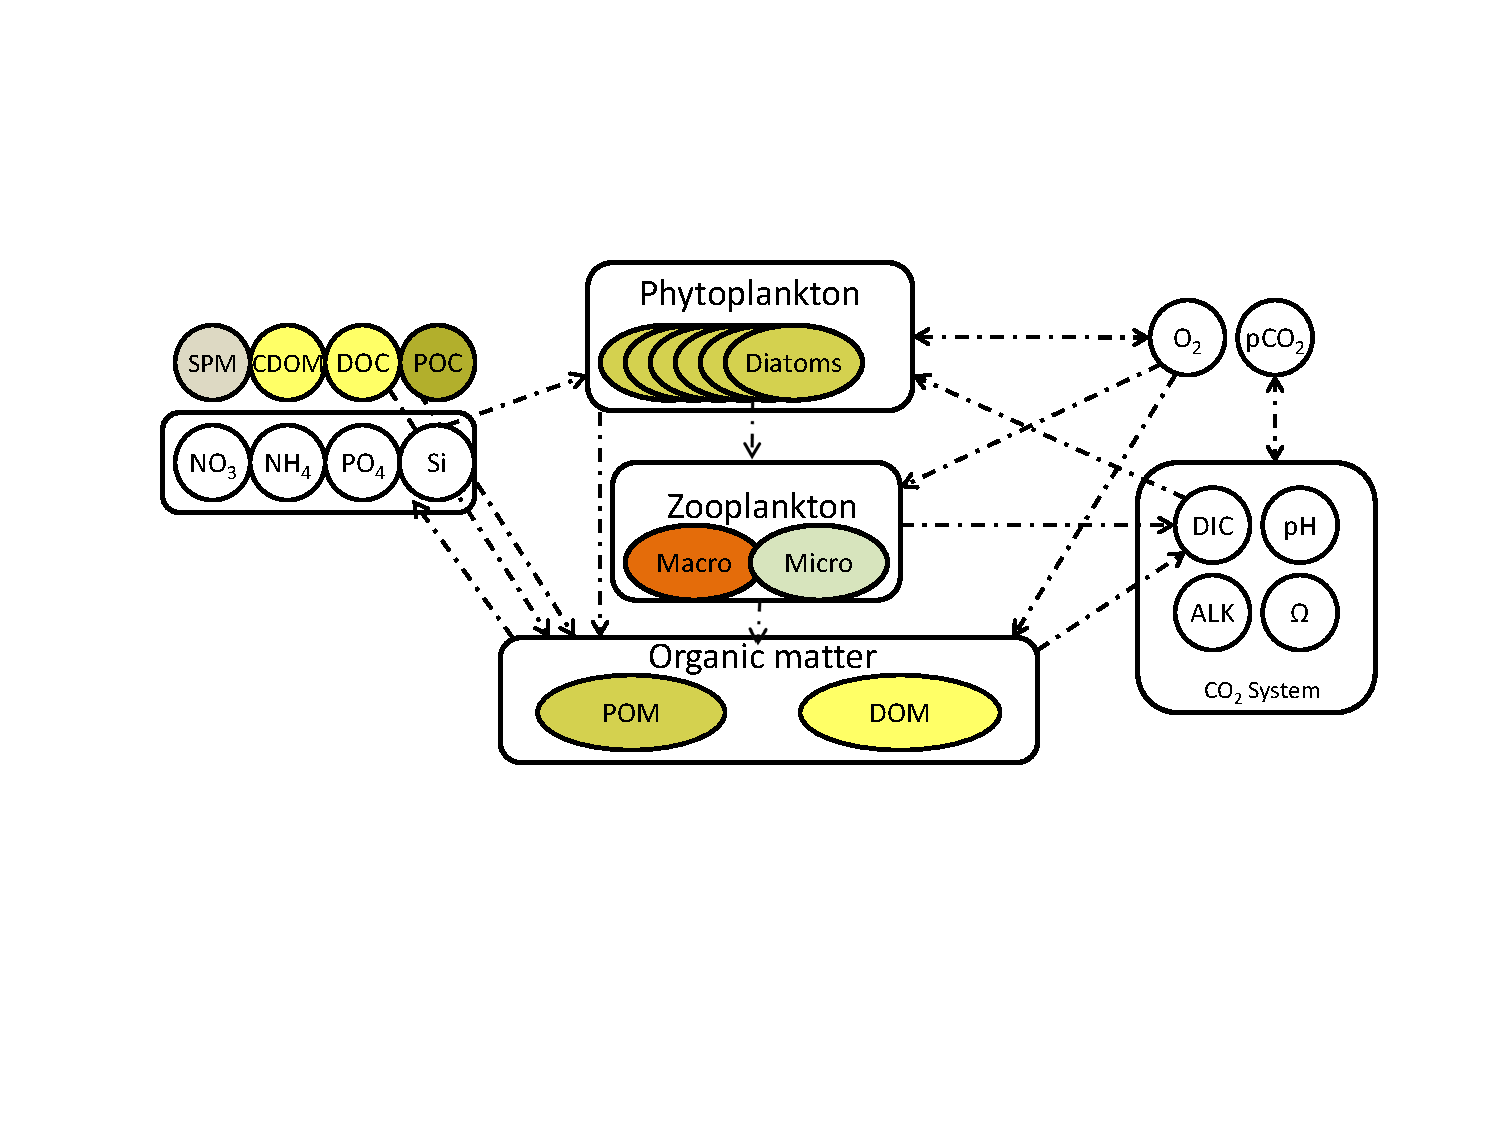
\includegraphics[width=0.7\textwidth]{figs/fishmod.pdf}
\caption{Conceptual representation of biogeochemical components included in FishTank (complete equations in \citealt{Eldridge10}). The \acl{cgem} couples FishTank with a hydrodynamic model that includes advection, mixing, and dispersion.}
\label{fig:fishmod}
\end{figure}

% combination example
\begin{figure}[!ht]

{\centering 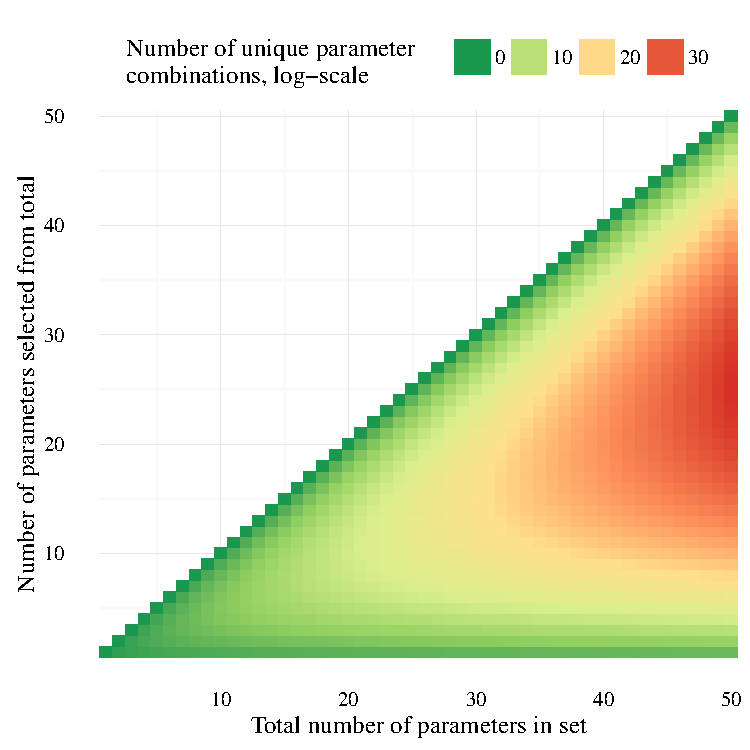
\includegraphics[width=0.6\textwidth]{figs/combnex-1} 

}

\caption[Examples of unique parameter combinations from different parameter sets and number of selected parameters]{Examples of unique parameter combinations from different parameter sets and number of selected parameters.  The number of combinations are shown for increasing numbers of selected parameters from the total in the set, where 50 parameter sets are shown each with one through 50 total parameters. Note that the number of unique combinations is shown as the natural-log.}\label{fig:combnex}
\end{figure}



% sensitivity heat map
\begin{figure}[!ht]

{\centering 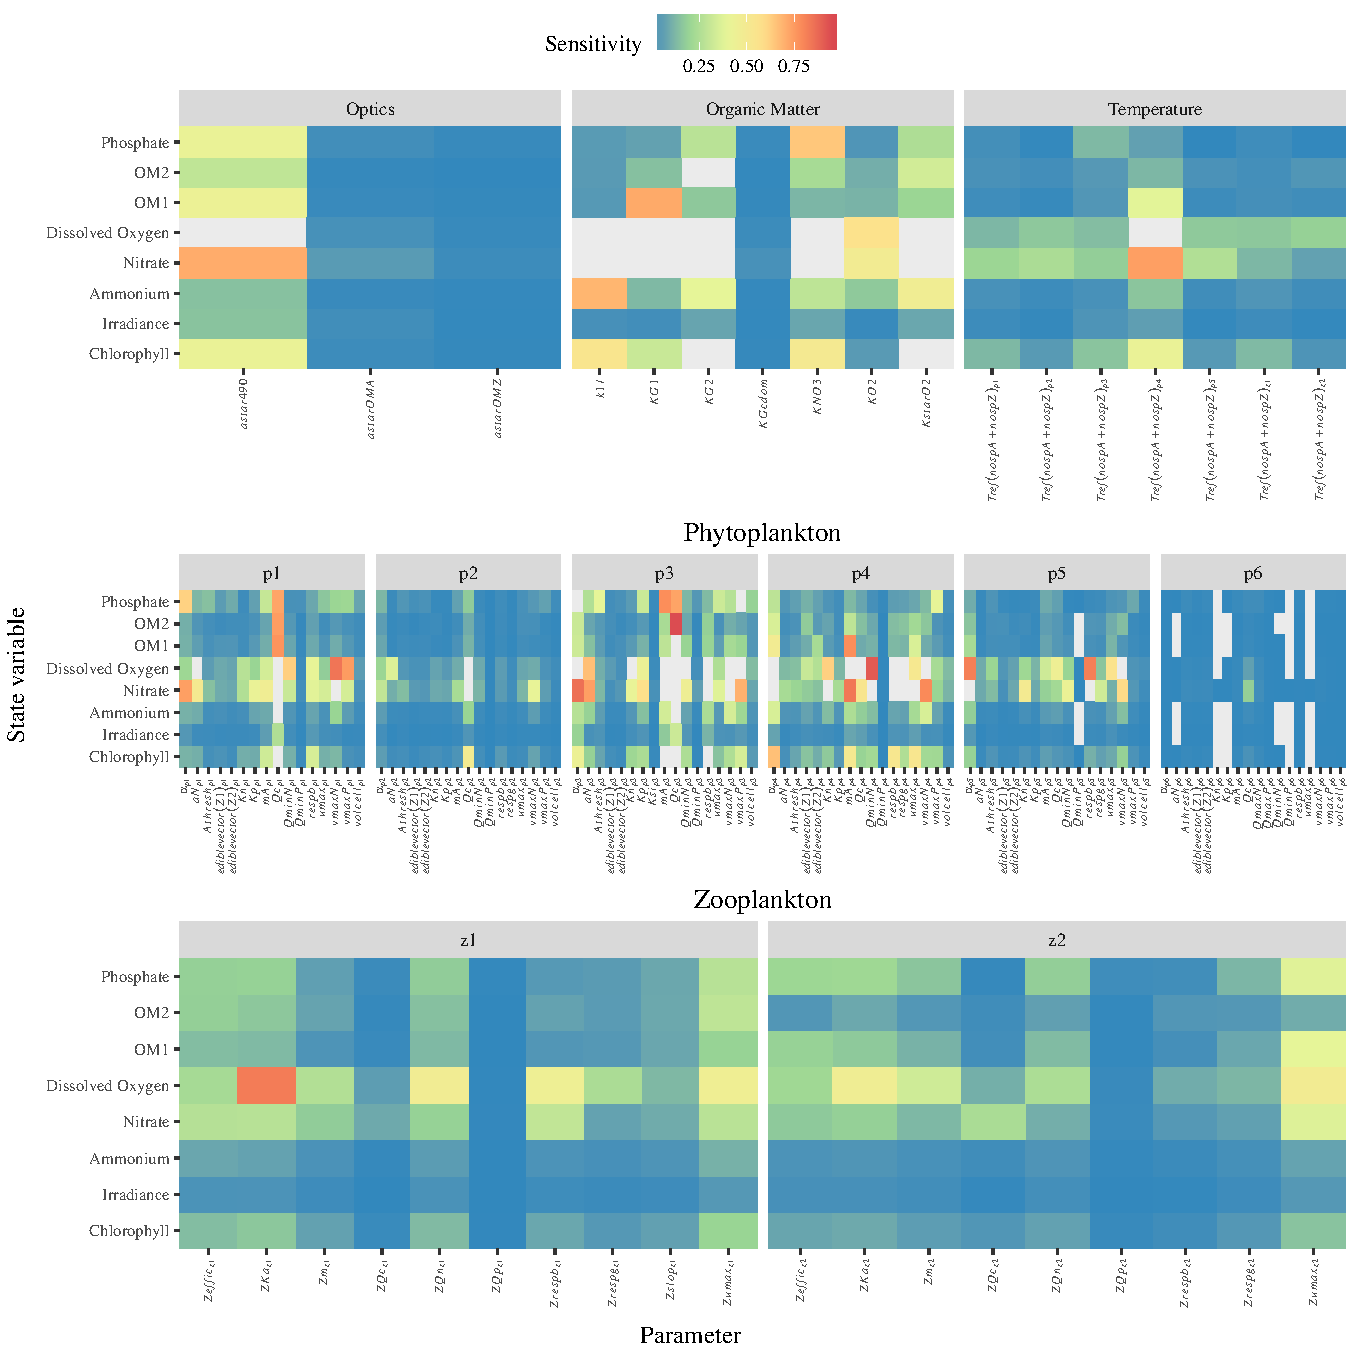
\includegraphics[width=0.7\textwidth]{figs/sensalltile-1} 

}

\caption{Sensitivity values (L1, \cref{l1}) of all state variables to changes in a 50\% increase in parameter values. Parameters are grouped by category: optics, organic matter, phytoplankton, zooplankton, temperature, and zoplankton.  See \cref{tab:dosens} for L1 values for \ac{do} and \cref{tab:nh4sens,tab:chlsens,tab:irrsens,tab:no3sens,tab:om1sens,tab:om2sens,tab:po4sens} for the other state variables.}\label{fig:sensalltile}
\end{figure}



% identifiability plot
\begin{figure}[!ht]

{\centering 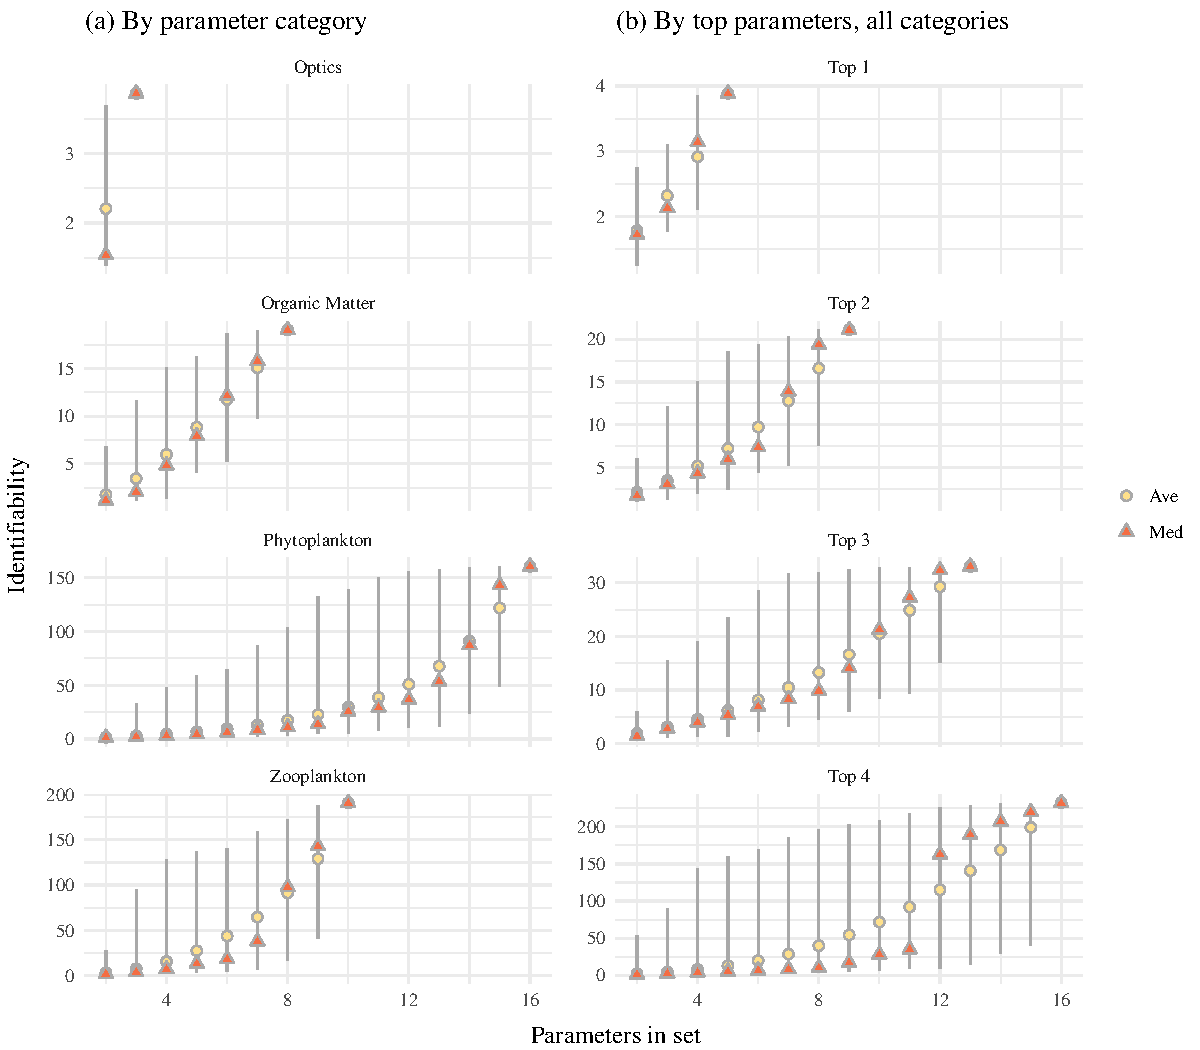
\includegraphics[width=\maxwidth]{figs/identplo-1} 

}

\caption{Collinearity ($\gamma$ as a measure of identifiability, \cref{gameq}) of parameter subsets for \ac{do}.  Plots in (a) show collinearity by parameter categories and (b) shows collinearity by selecting the top 1 through 4 parameters in all categories.  Lines represent collinearity ranges for the possible combinations given the number of parameters in the set.  The temperature category is not shown because \ac{do} was sensitive to only one parameter (i.e., $\gamma = 1$).}\label{fig:identplo}
\end{figure}



% identifiability plot, all state variables
\begin{figure}[!ht]

{\centering 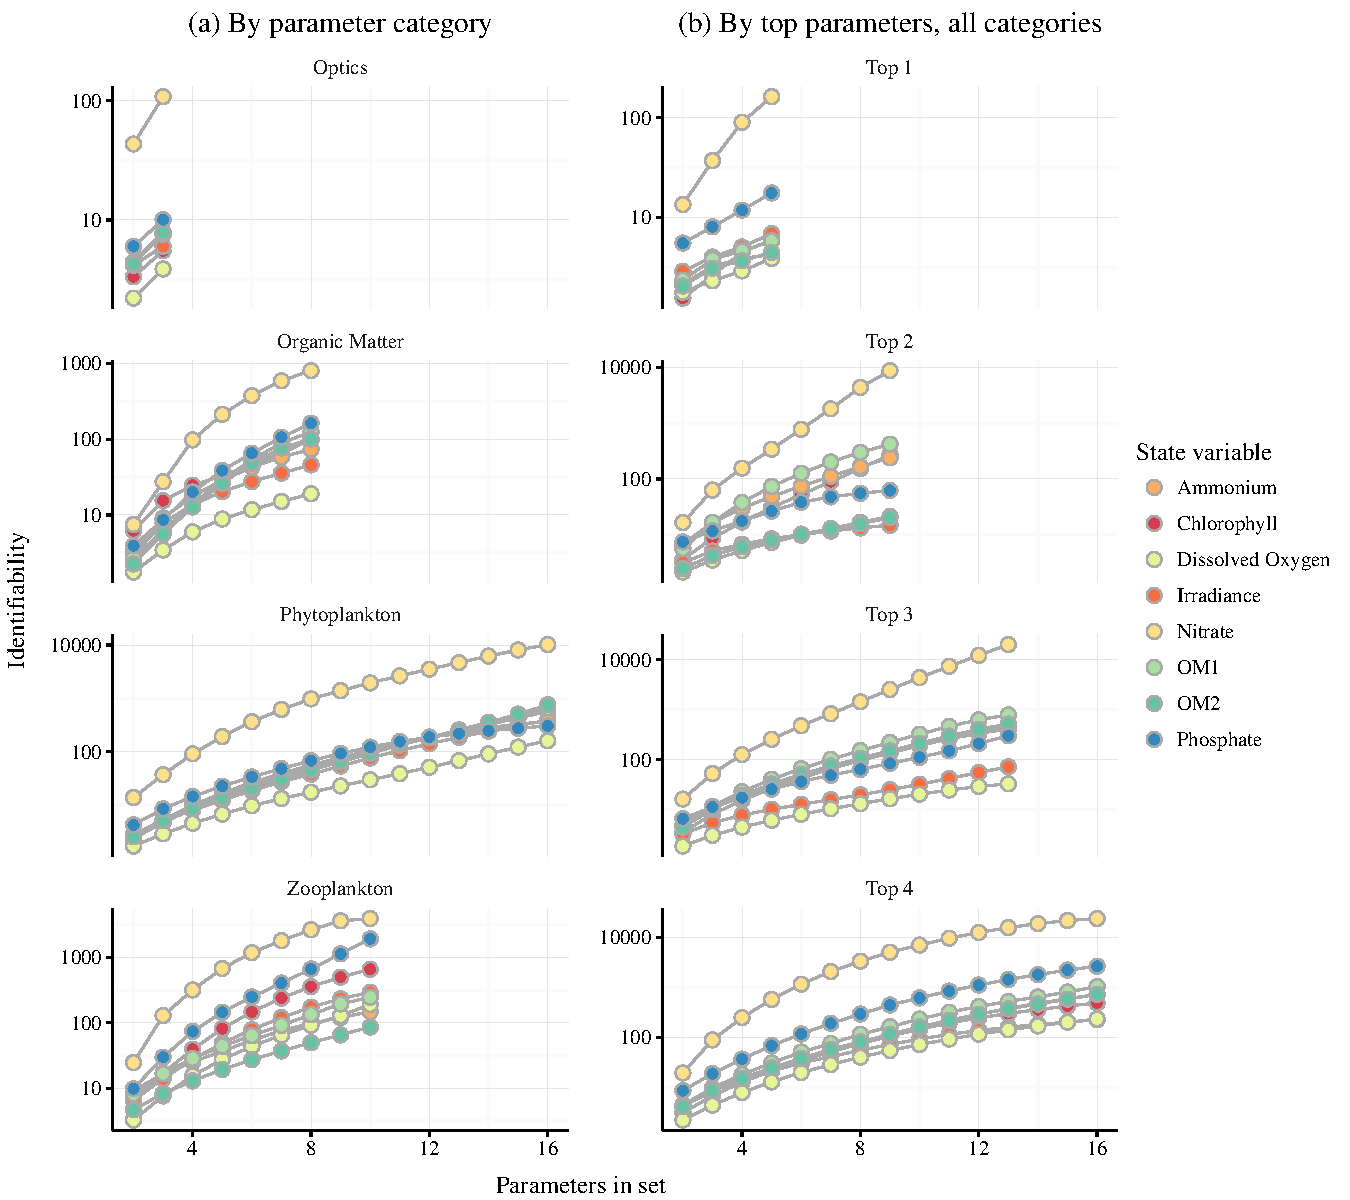
\includegraphics[width=\maxwidth]{figs/identploall-1} 

}

\caption[Average collinearity ($\gamma$ as a measure of identifiability, \cref{gameq}) of parameter subsets for all state variables]{Average collinearity ($\gamma$ as a measure of identifiability, \cref{gameq}) of parameter subsets for all state variables.  Plots in (a) show collinearity by parameter categories and (b) shows collinearity by selecting the top 1 through 4 parameters in all categories.  Collinearity was averaged for all combinations in a parameter set to evaluate relative differenes between state variables.  The temperature category is not shown because all state variables were sensitive to only one parameter (i.e., $\gamma = 1$).}\label{fig:identploall}
\end{figure}



% parameter exclusion temp
\begin{figure}[!ht]

{\centering 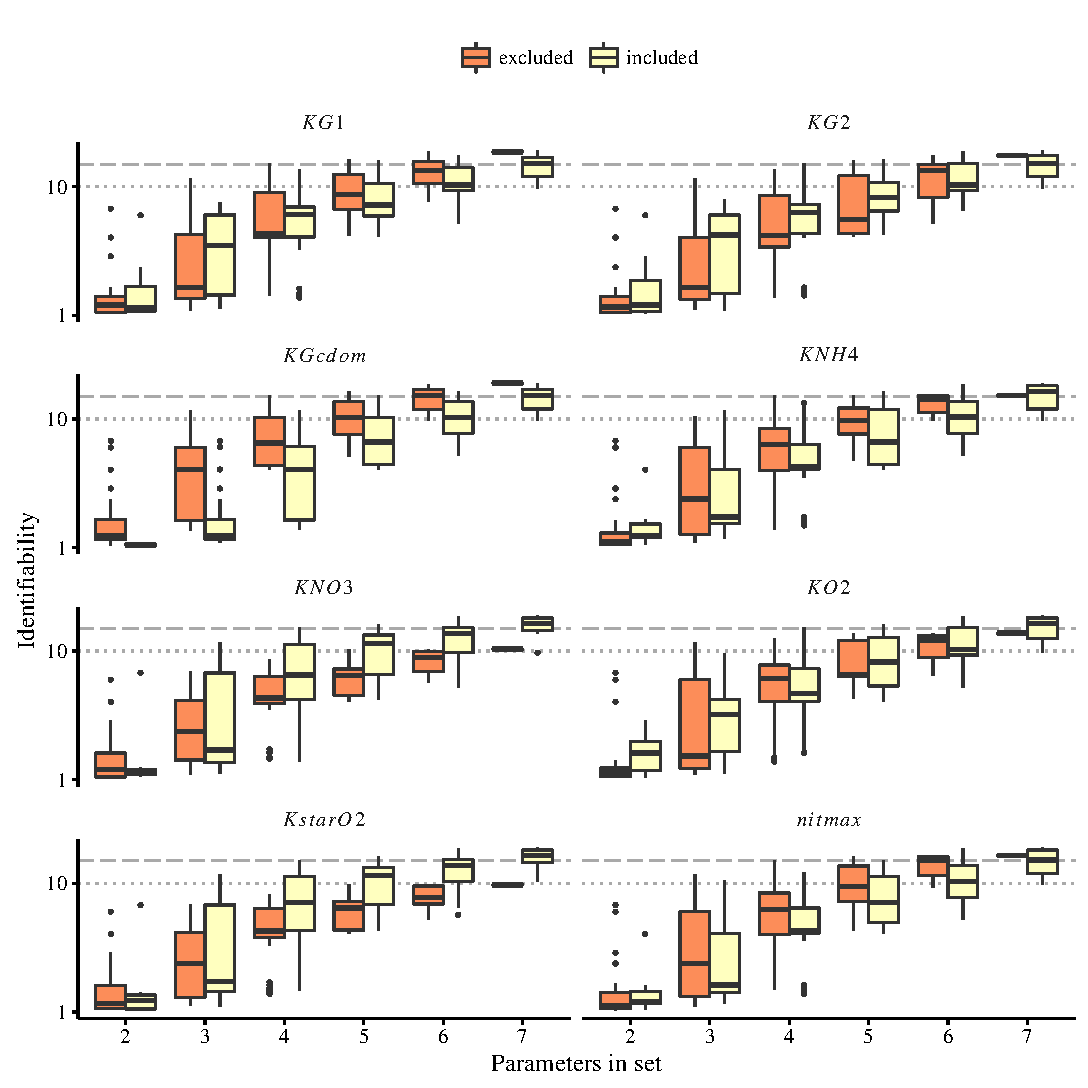
\includegraphics[width=0.8\textwidth]{figs/exclex-1} 

}

\caption{Collinearity ($\gamma$ as a measure of identifiability, \cref{gameq}) for \ac{do} of organic matter parameters for subset combinations in \cref{fig:identplo}.  Collinearity is evaluated for subsets that excluded and included the parameters at the top of each plot. Collinearity of including all eight parameters is in \cref{fig:identplo}. Grey lines indicate potential thresholds at $\gamma = 10, 15$ for maximum acceptable collinearity.}\label{fig:exclex}
\end{figure}



% calibration example
\begin{figure}[!ht]

{\centering 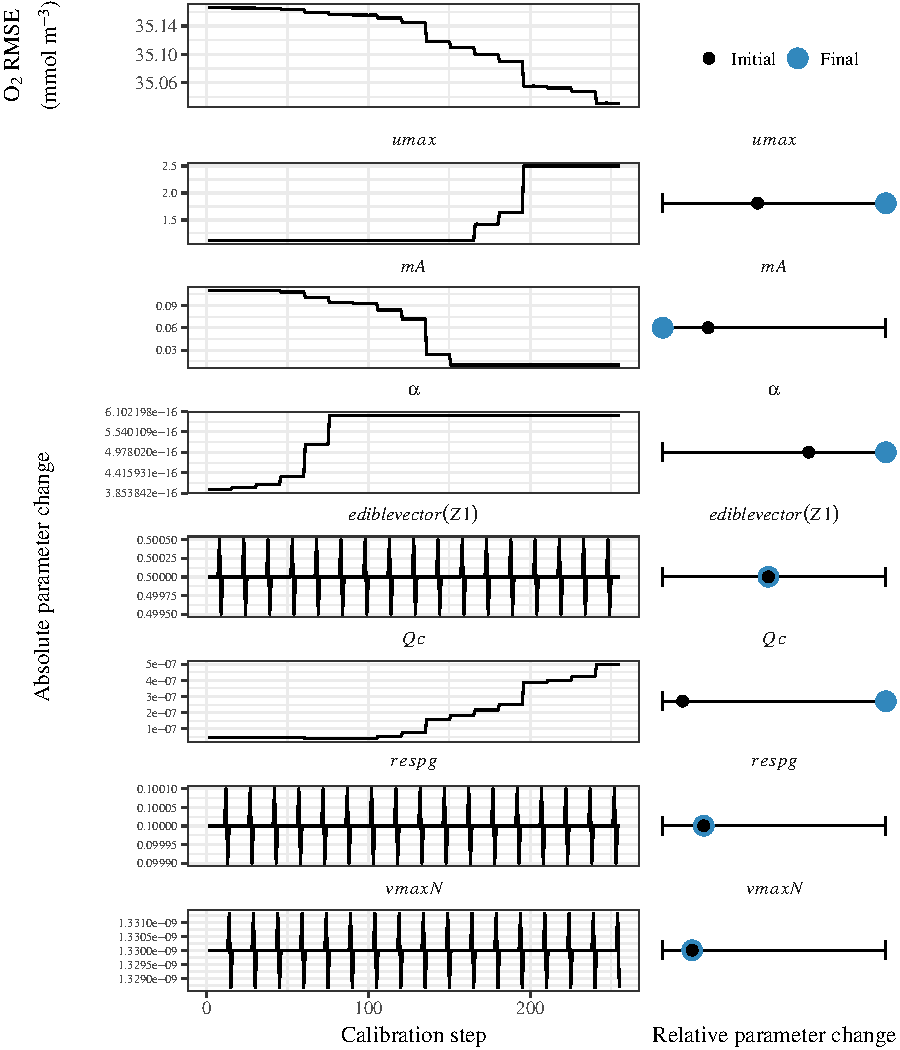
\includegraphics[width=\textwidth]{figs/calex-1} 

}

\caption{Example of calibration steps for the phytoplankton parameter subset.  The FishTank model was calibrated using data from an approximate 12-hour flask experiment of oxygen production.  Model calibration adjusted parameters (left plots) to minimize the \ac{rmse} between experimental and modelled dissolved oxygen (top left).  The phytoplankton parameters were those identifiable for dissolved oxygen (\cref{tab:heurist1}), arranged from most (top plot) to least sensitive (bottom plot) (\cref{tab:dosens}).  The relative parameter changes in the right plots show the initial parameter values (black) and the the selected parameter values (blue) after calibration.}\label{fig:calex}
\end{figure}



% CGEM area change plots
\begin{figure}[!ht]

{\centering 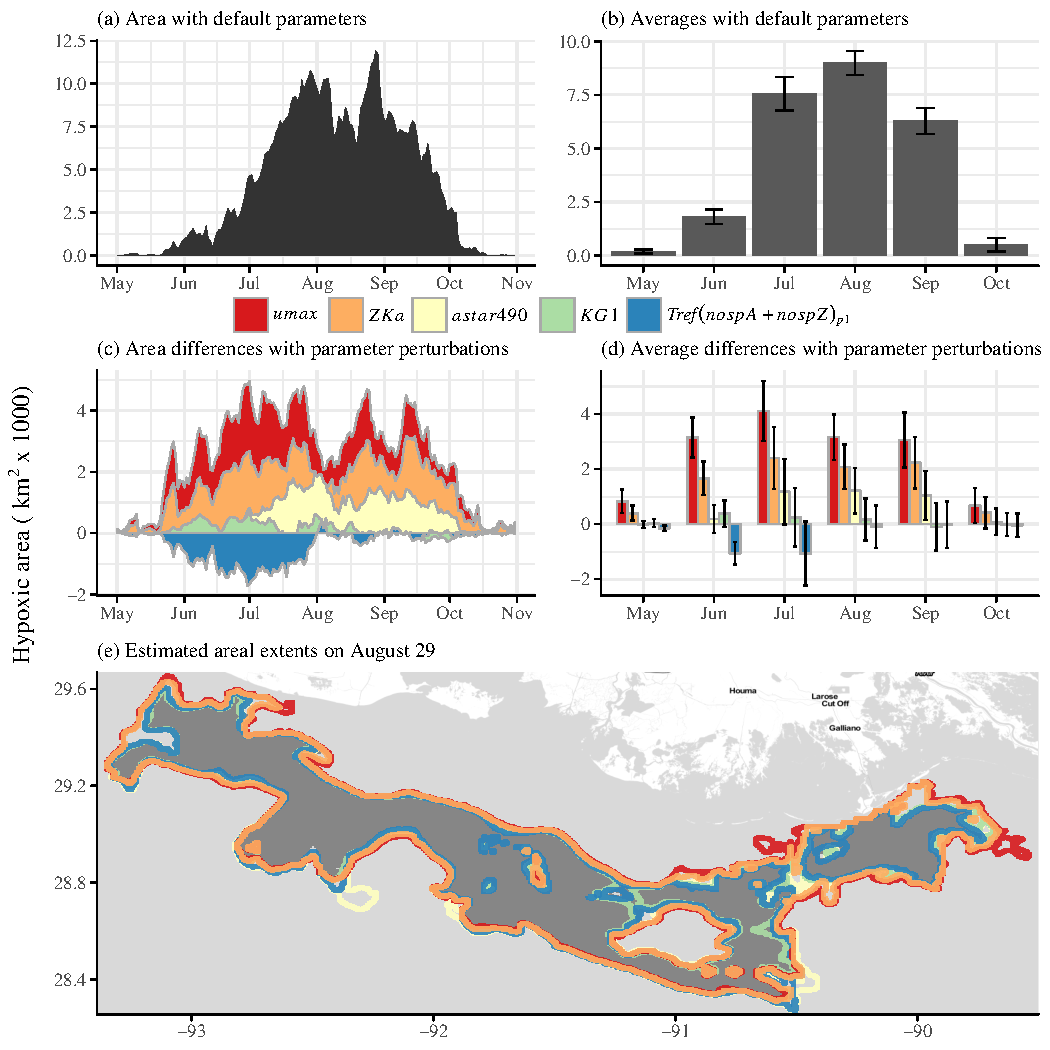
\includegraphics[width=\textwidth]{figs/areachg-1} 

}

\caption{Estimated hypoxic area and monthly averages (km$^2 \times$ 1000) using the default parameter settings (a, b) and the differences using a 50\% increase in each parameter (c, d).  The selected parameters were the top sensitive in each parameter category for \ac{do} in \cref{fig:sensalltile,tab:dosens}. Error bars are 95\% confidence intervals for the monthly averages in (b) and the difference in monthly averages (d) from the perturbed and default results.  Areal extent of estimated hypoxia on August 28\textsuperscript{th} using the default parameters (grey) and estimated changes with parameter perturbations is shown in (e).}\label{fig:areachg}
\end{figure}



\clearpage

% supplementary material
\beginsupplement

%%
% sup tabs

% ammonium sensitivity all categories
%latex.default(totab, file = "", rowlabel = "Description", caption = cap.val,     caption.loc = "top", rowname = Description, rgroup = unique(cats),     n.rgroup = as.numeric(table(cats)), size = tabsize, label = paste0("tab:",         tablab), insert.bottom = foot.val)%
\begin{table}[!tbp]
{\footnotesize
\caption{Sensitivity of ammonium to perturbations of individual parameters.  Sensitivities are based on a 50\% increase from the initial parameter value, where $L1$ summarizes differences in model output (see \cref{l1}).  Parameters that did not affect ammonium are not shown.  Parameters are grouped by categories as optics, temperature, phytoplankton, zooplankton, and organic matter.\label{tab:nh4sens}} 
\begin{center}
\begin{tabular}{lll}
\hline\hline
\multicolumn{1}{l}{Description}&\multicolumn{1}{c}{Parameter}&\multicolumn{1}{c}{L1}\tabularnewline
\hline
{\bfseries Optics}&&\tabularnewline
~~Chla specific absorption at 490 nm&\textit{astar490}&$0.03$\tabularnewline
~~OMA specific absorption at 490 nm&\textit{astarOMA}&$1.63\times 10^{-3}$\tabularnewline
~~OMZ specific absorption at 490 nm&\textit{astarOMZ}&$1.5\times 10^{-3}$\tabularnewline
\hline
{\bfseries Organic Matter}&&\tabularnewline
~~maximum rate of nitrification per day&\textit{nitmax}&$1.54$\tabularnewline
~~NH4 rate constant for nitrification&\textit{KNH4}&$0.66$\tabularnewline
~~turnover rate for OM1A and OM1Z&\textit{KG1}&$0.07$\tabularnewline
~~decay rate of CDOM&\textit{KGcdom}&$0.07$\tabularnewline
~~half-saturation concentration for O2 utilization&\textit{KO2}&$0.06$\tabularnewline
~~O2 concentration that inhibits denitrification&\textit{KstarO2}&$0.05$\tabularnewline
~~turnover rate for OM2A and OM2Z&\textit{KG2}&$0.03$\tabularnewline
~~half-saturation concentration for denitrification&\textit{KNO3}&$7.55\times 10^{-3}$\tabularnewline
\hline
{\bfseries Phytoplankton}&&\tabularnewline
~~mortality coefficient&\textit{mA}&$8.49$\tabularnewline
~~edibility vector for Z1&\textit{ediblevector(Z1)}&$1.32$\tabularnewline
~~maximum growth rate&\textit{umax}&$0.65$\tabularnewline
~~initial slope of photosynthesis v irradiance&\textit{alpha}&$0.6$\tabularnewline
~~N-uptake rate measured at umax&\textit{vmaxN}&$0.46$\tabularnewline
~~phytoplankton threshold for grazing&\textit{Athresh}&$0.29$\tabularnewline
~~coefficient for non-limiting nutrient&\textit{aN}&$0.17$\tabularnewline
~~phytoplankton growth respiration coefficient&\textit{respg}&$0.16$\tabularnewline
~~phytoplankton basal respiration coefficient&\textit{respb}&$0.15$\tabularnewline
~~half-saturation constant for P&\textit{Kp}&$0.14$\tabularnewline
~~phytoplankton volume/cell&\textit{volcell}&$0.14$\tabularnewline
~~minimum N cell-quota&\textit{QminN}&$0.1$\tabularnewline
~~P-uptake rate measured at umax&\textit{vmaxP}&$0.1$\tabularnewline
~~phytoplankton carbon/cell&\textit{Qc}&$0.03$\tabularnewline
~~half-saturation constant for N&\textit{Kn}&$0.01$\tabularnewline
~~minimum P cell-quota&\textit{QminP}&$2.24\times 10^{-6}$\tabularnewline
\hline
{\bfseries Temperature}&&\tabularnewline
~~Optimum temperature for growth&\textit{Tref(nospA+nospZ)$_{p1}$}&$0.79$\tabularnewline
\hline
{\bfseries Zooplankton}&&\tabularnewline
~~maximum growth rate of zooplankton&\textit{Zumax}&$1.42$\tabularnewline
~~assimilation efficiency as a fraction of ingestion&\textit{Zeffic}&$0.76$\tabularnewline
~~half saturation coefficient for grazing&\textit{ZKa}&$0.74$\tabularnewline
~~zooplankton nitrogen/individual&\textit{ZQn}&$0.62$\tabularnewline
~~quadratic mortality constant&\textit{Zm}&$0.5$\tabularnewline
~~proportion of phytoplankton lost to sloppy feeding&\textit{Zslop}&$0.3$\tabularnewline
~~zooplankton growth-dependent respiration factor&\textit{Zrespg}&$0.22$\tabularnewline
~~zooplankton biomass-dependent respiration factor&\textit{Zrespb}&$0.16$\tabularnewline
~~zooplankton phosphorus/individual&\textit{ZQp}&$1.07\times 10^{-3}$\tabularnewline
~~zooplankton carbon/individual&\textit{ZQc}&$1.44\times 10^{-4}$\tabularnewline
\hline
\end{tabular}\end{center}}
\end{table}


% chlorophyll sensitivity all categories
%latex.default(totab, file = "", rowlabel = "Description", caption = cap.val,     caption.loc = "top", rowname = Description, rgroup = unique(cats),     n.rgroup = as.numeric(table(cats)), size = tabsize, label = paste0("tab:",         tablab), insert.bottom = foot.val)%
\begin{table}[!tbp]
{\footnotesize
\caption{Sensitivity of \ac{chla} to perturbations of individual parameters.  Sensitivities are based on a 50\% increase from the initial parameter value, where $L1$ summarizes differences in model output (see \cref{l1}).  Parameters that did not affect \ac{chla} are not shown.  Parameters are grouped by categories as optics, temperature, phytoplankton, zooplankton, and organic matter.\label{tab:chlsens}} 
\begin{center}
\begin{tabular}{lll}
\hline\hline
\multicolumn{1}{l}{Description}&\multicolumn{1}{c}{Parameter}&\multicolumn{1}{c}{L1}\tabularnewline
\hline
{\bfseries Optics}&&\tabularnewline
~~Chla specific absorption at 490 nm&\textit{astar490}&$0.02$\tabularnewline
~~OMA specific absorption at 490 nm&\textit{astarOMA}&$1.45\times 10^{-3}$\tabularnewline
~~OMZ specific absorption at 490 nm&\textit{astarOMZ}&$1.13\times 10^{-3}$\tabularnewline
\hline
{\bfseries Organic Matter}&&\tabularnewline
~~decay rate of CDOM&\textit{KGcdom}&$0.07$\tabularnewline
~~turnover rate for OM1A and OM1Z&\textit{KG1}&$0.03$\tabularnewline
~~turnover rate for OM2A and OM2Z&\textit{KG2}&$0.01$\tabularnewline
~~O2 concentration that inhibits denitrification&\textit{KstarO2}&$0.01$\tabularnewline
~~half-saturation concentration for O2 utilization&\textit{KO2}&$3.35\times 10^{-3}$\tabularnewline
~~half-saturation concentration for denitrification&\textit{KNO3}&$1.19\times 10^{-3}$\tabularnewline
~~maximum rate of nitrification per day&\textit{nitmax}&$3.4\times 10^{-5}$\tabularnewline
~~NH4 rate constant for nitrification&\textit{KNH4}&$2.97\times 10^{-5}$\tabularnewline
\hline
{\bfseries Phytoplankton}&&\tabularnewline
~~mortality coefficient&\textit{mA}&$13.94$\tabularnewline
~~edibility vector for Z1&\textit{ediblevector(Z1)}&$0.95$\tabularnewline
~~maximum growth rate&\textit{umax}&$0.85$\tabularnewline
~~initial slope of photosynthesis v irradiance&\textit{alpha}&$0.62$\tabularnewline
~~N-uptake rate measured at umax&\textit{vmaxN}&$0.53$\tabularnewline
~~phytoplankton growth respiration coefficient&\textit{respg}&$0.26$\tabularnewline
~~phytoplankton threshold for grazing&\textit{Athresh}&$0.25$\tabularnewline
~~phytoplankton basal respiration coefficient&\textit{respb}&$0.24$\tabularnewline
~~coefficient for non-limiting nutrient&\textit{aN}&$0.17$\tabularnewline
~~half-saturation constant for P&\textit{Kp}&$0.14$\tabularnewline
~~P-uptake rate measured at umax&\textit{vmaxP}&$0.12$\tabularnewline
~~phytoplankton volume/cell&\textit{volcell}&$0.1$\tabularnewline
~~minimum N cell-quota&\textit{QminN}&$0.07$\tabularnewline
~~phytoplankton carbon/cell&\textit{Qc}&$0.02$\tabularnewline
~~half-saturation constant for N&\textit{Kn}&$0.01$\tabularnewline
~~minimum P cell-quota&\textit{QminP}&$1.38\times 10^{-6}$\tabularnewline
\hline
{\bfseries Temperature}&&\tabularnewline
~~Optimum temperature for growth&\textit{Tref(nospA+nospZ)$_{p1}$}&$0.6$\tabularnewline
\hline
{\bfseries Zooplankton}&&\tabularnewline
~~maximum growth rate of zooplankton&\textit{Zumax}&$1.02$\tabularnewline
~~half saturation coefficient for grazing&\textit{ZKa}&$0.85$\tabularnewline
~~assimilation efficiency as a fraction of ingestion&\textit{Zeffic}&$0.57$\tabularnewline
~~zooplankton nitrogen/individual&\textit{ZQn}&$0.52$\tabularnewline
~~quadratic mortality constant&\textit{Zm}&$0.41$\tabularnewline
~~proportion of phytoplankton lost to sloppy feeding&\textit{Zslop}&$0.23$\tabularnewline
~~zooplankton growth-dependent respiration factor&\textit{Zrespg}&$0.17$\tabularnewline
~~zooplankton biomass-dependent respiration factor&\textit{Zrespb}&$0.14$\tabularnewline
~~zooplankton phosphorus/individual&\textit{ZQp}&$1.29\times 10^{-3}$\tabularnewline
~~zooplankton carbon/individual&\textit{ZQc}&$7.55\times 10^{-5}$\tabularnewline
\hline
\end{tabular}\end{center}}
\end{table}


% irradiance sensitivity all categories
%latex.default(totab, file = "", rowlabel = "Description", caption = cap.val,     caption.loc = "top", rowname = Description, rgroup = unique(cats),     n.rgroup = as.numeric(table(cats)), size = tabsize, label = paste0("tab:",         tablab), insert.bottom = foot.val)%
\begin{table}[!tbp]
{\footnotesize
\caption{Sensitivity of irradiance to perturbations of individual parameters.  Sensitivities are based on a 50\% increase from the initial parameter value, where $L1$ summarizes differences in model output (see \cref{l1}).  Parameters that did not affect irradiance are not shown.  Parameters are grouped by categories as optics, temperature, phytoplankton, zooplankton, and organic matter.\label{tab:irrsens}} 
\begin{center}
\begin{tabular}{lll}
\hline\hline
\multicolumn{1}{l}{Description}&\multicolumn{1}{c}{Parameter}&\multicolumn{1}{c}{L1}\tabularnewline
\hline
{\bfseries Optics}&&\tabularnewline
~~Chla specific absorption at 490 nm&\textit{astar490}&$0.02$\tabularnewline
~~OMA specific absorption at 490 nm&\textit{astarOMA}&$1.47\times 10^{-3}$\tabularnewline
~~OMZ specific absorption at 490 nm&\textit{astarOMZ}&$1.34\times 10^{-3}$\tabularnewline
\hline
{\bfseries Organic Matter}&&\tabularnewline
~~decay rate of CDOM&\textit{KGcdom}&$0.05$\tabularnewline
~~turnover rate for OM1A and OM1Z&\textit{KG1}&$3.96\times 10^{-3}$\tabularnewline
~~turnover rate for OM2A and OM2Z&\textit{KG2}&$9.88\times 10^{-4}$\tabularnewline
~~O2 concentration that inhibits denitrification&\textit{KstarO2}&$7.2\times 10^{-4}$\tabularnewline
~~half-saturation concentration for O2 utilization&\textit{KO2}&$3.54\times 10^{-4}$\tabularnewline
~~half-saturation concentration for denitrification&\textit{KNO3}&$6.18\times 10^{-5}$\tabularnewline
~~maximum rate of nitrification per day&\textit{nitmax}&$1.72\times 10^{-6}$\tabularnewline
~~NH4 rate constant for nitrification&\textit{KNH4}&$1.48\times 10^{-6}$\tabularnewline
\hline
{\bfseries Phytoplankton}&&\tabularnewline
~~maximum growth rate&\textit{umax}&$0.09$\tabularnewline
~~mortality coefficient&\textit{mA}&$0.05$\tabularnewline
~~initial slope of photosynthesis v irradiance&\textit{alpha}&$0.04$\tabularnewline
~~edibility vector for Z1&\textit{ediblevector(Z1)}&$0.04$\tabularnewline
~~N-uptake rate measured at umax&\textit{vmaxN}&$0.03$\tabularnewline
~~phytoplankton threshold for grazing&\textit{Athresh}&$0.02$\tabularnewline
~~coefficient for non-limiting nutrient&\textit{aN}&$0.01$\tabularnewline
~~phytoplankton growth respiration coefficient&\textit{respg}&$0.01$\tabularnewline
~~half-saturation constant for P&\textit{Kp}&$0.01$\tabularnewline
~~P-uptake rate measured at umax&\textit{vmaxP}&$9.48\times 10^{-3}$\tabularnewline
~~phytoplankton basal respiration coefficient&\textit{respb}&$9.38\times 10^{-3}$\tabularnewline
~~phytoplankton volume/cell&\textit{volcell}&$8.1\times 10^{-3}$\tabularnewline
~~minimum N cell-quota&\textit{QminN}&$5.75\times 10^{-3}$\tabularnewline
~~phytoplankton carbon/cell&\textit{Qc}&$3.78\times 10^{-3}$\tabularnewline
~~half-saturation constant for N&\textit{Kn}&$9.81\times 10^{-4}$\tabularnewline
~~minimum P cell-quota&\textit{QminP}&$1.92\times 10^{-7}$\tabularnewline
\hline
{\bfseries Temperature}&&\tabularnewline
~~Optimum temperature for growth&\textit{Tref(nospA+nospZ)$_{p1}$}&$0.03$\tabularnewline
\hline
{\bfseries Zooplankton}&&\tabularnewline
~~half saturation coefficient for grazing&\textit{ZKa}&$0.13$\tabularnewline
~~zooplankton nitrogen/individual&\textit{ZQn}&$0.06$\tabularnewline
~~maximum growth rate of zooplankton&\textit{Zumax}&$0.04$\tabularnewline
~~quadratic mortality constant&\textit{Zm}&$0.04$\tabularnewline
~~assimilation efficiency as a fraction of ingestion&\textit{Zeffic}&$0.03$\tabularnewline
~~proportion of phytoplankton lost to sloppy feeding&\textit{Zslop}&$0.02$\tabularnewline
~~zooplankton growth-dependent respiration factor&\textit{Zrespg}&$0.01$\tabularnewline
~~zooplankton biomass-dependent respiration factor&\textit{Zrespb}&$9.67\times 10^{-3}$\tabularnewline
~~zooplankton phosphorus/individual&\textit{ZQp}&$9.34\times 10^{-5}$\tabularnewline
~~zooplankton carbon/individual&\textit{ZQc}&$1.99\times 10^{-5}$\tabularnewline
\hline
\end{tabular}\end{center}}
\end{table}


% nitrate sensitivity all categories
%latex.default(totab, file = "", rowlabel = "Description", caption = cap.val,     caption.loc = "top", rowname = Description, rgroup = unique(cats),     n.rgroup = as.numeric(table(cats)), size = tabsize, label = paste0("tab:",         tablab), insert.bottom = foot.val)%
\begin{table}[!tbp]
{\footnotesize
\caption{Sensitivity of nitrate to perturbations of individual parameters.  Sensitivities are based on a 50\% increase from the initial parameter value, where $L1$ summarizes differences in model output (see \cref{l1}).  Parameters that did not affect nitrate are not shown.  Parameters are grouped by categories as optics, temperature, phytoplankton, zooplankton, and organic matter.\label{tab:no3sens}} 
\begin{center}
\begin{tabular}{lll}
\hline\hline
\multicolumn{1}{l}{Description}&\multicolumn{1}{c}{Parameter}&\multicolumn{1}{c}{L1}\tabularnewline
\hline
{\bfseries Optics}&&\tabularnewline
~~Chla specific absorption at 490 nm&\textit{astar490}&$0.02$\tabularnewline
~~OMZ specific absorption at 490 nm&\textit{astarOMZ}&$1.27\times 10^{-3}$\tabularnewline
~~OMA specific absorption at 490 nm&\textit{astarOMA}&$1.19\times 10^{-3}$\tabularnewline
\hline
{\bfseries Organic Matter}&&\tabularnewline
~~O2 concentration that inhibits denitrification&\textit{KstarO2}&$0.78$\tabularnewline
~~half-saturation concentration for denitrification&\textit{KNO3}&$0.07$\tabularnewline
~~decay rate of CDOM&\textit{KGcdom}&$0.04$\tabularnewline
~~half-saturation concentration for O2 utilization&\textit{KO2}&$0.03$\tabularnewline
~~turnover rate for OM1A and OM1Z&\textit{KG1}&$0.02$\tabularnewline
~~turnover rate for OM2A and OM2Z&\textit{KG2}&$0.01$\tabularnewline
~~maximum rate of nitrification per day&\textit{nitmax}&$9.96\times 10^{-3}$\tabularnewline
~~NH4 rate constant for nitrification&\textit{KNH4}&$9.87\times 10^{-3}$\tabularnewline
\hline
{\bfseries Phytoplankton}&&\tabularnewline
~~maximum growth rate&\textit{umax}&$8.49$\tabularnewline
~~phytoplankton carbon/cell&\textit{Qc}&$0.89$\tabularnewline
~~initial slope of photosynthesis v irradiance&\textit{alpha}&$0.7$\tabularnewline
~~edibility vector for Z1&\textit{ediblevector(Z1)}&$0.33$\tabularnewline
~~mortality coefficient&\textit{mA}&$0.27$\tabularnewline
~~phytoplankton threshold for grazing&\textit{Athresh}&$0.2$\tabularnewline
~~N-uptake rate measured at umax&\textit{vmaxN}&$0.19$\tabularnewline
~~coefficient for non-limiting nutrient&\textit{aN}&$0.13$\tabularnewline
~~phytoplankton growth respiration coefficient&\textit{respg}&$0.11$\tabularnewline
~~phytoplankton volume/cell&\textit{volcell}&$0.1$\tabularnewline
~~P-uptake rate measured at umax&\textit{vmaxP}&$0.1$\tabularnewline
~~half-saturation constant for P&\textit{Kp}&$0.09$\tabularnewline
~~minimum N cell-quota&\textit{QminN}&$0.09$\tabularnewline
~~phytoplankton basal respiration coefficient&\textit{respb}&$0.07$\tabularnewline
~~half-saturation constant for N&\textit{Kn}&$7.06\times 10^{-3}$\tabularnewline
~~minimum P cell-quota&\textit{QminP}&$6.67\times 10^{-7}$\tabularnewline
\hline
{\bfseries Temperature}&&\tabularnewline
~~Optimum temperature for growth&\textit{Tref(nospA+nospZ)$_{p1}$}&$0.3$\tabularnewline
\hline
{\bfseries Zooplankton}&&\tabularnewline
~~half saturation coefficient for grazing&\textit{ZKa}&$7.59$\tabularnewline
~~zooplankton nitrogen/individual&\textit{ZQn}&$1.17$\tabularnewline
~~quadratic mortality constant&\textit{Zm}&$0.7$\tabularnewline
~~maximum growth rate of zooplankton&\textit{Zumax}&$0.34$\tabularnewline
~~proportion of phytoplankton lost to sloppy feeding&\textit{Zslop}&$0.26$\tabularnewline
~~assimilation efficiency as a fraction of ingestion&\textit{Zeffic}&$0.25$\tabularnewline
~~zooplankton growth-dependent respiration factor&\textit{Zrespg}&$0.17$\tabularnewline
~~zooplankton biomass-dependent respiration factor&\textit{Zrespb}&$0.1$\tabularnewline
~~zooplankton carbon/individual&\textit{ZQc}&$3.8\times 10^{-3}$\tabularnewline
~~zooplankton phosphorus/individual&\textit{ZQp}&$8.59\times 10^{-4}$\tabularnewline
\hline
\end{tabular}\end{center}}
\end{table}


% om1 sensitivity all categories
%latex.default(totab, file = "", rowlabel = "Description", caption = cap.val,     caption.loc = "top", rowname = Description, rgroup = unique(cats),     n.rgroup = as.numeric(table(cats)), size = tabsize, label = paste0("tab:",         tablab), insert.bottom = foot.val)%
\begin{table}[!tbp]
{\footnotesize
\caption{Sensitivity of \ac{pom} to perturbations of individual parameters.  Sensitivities are based on a 50\% increase from the initial parameter value, where $L1$ summarizes differences in model output (see \cref{l1}).  Parameters that did not affect \ac{pom} are not shown.  Parameters are grouped by categories as optics, temperature, phytoplankton, zooplankton, and organic matter.\label{tab:om1sens}} 
\begin{center}
\begin{tabular}{lll}
\hline\hline
\multicolumn{1}{l}{Description}&\multicolumn{1}{c}{Parameter}&\multicolumn{1}{c}{L1}\tabularnewline
\hline
{\bfseries Optics}&&\tabularnewline
~~Chla specific absorption at 490 nm&\textit{astar490}&$0.03$\tabularnewline
~~OMA specific absorption at 490 nm&\textit{astarOMA}&$1.73\times 10^{-3}$\tabularnewline
~~OMZ specific absorption at 490 nm&\textit{astarOMZ}&$1.49\times 10^{-3}$\tabularnewline
\hline
{\bfseries Organic Matter}&&\tabularnewline
~~turnover rate for OM1A and OM1Z&\textit{KG1}&$0.92$\tabularnewline
~~decay rate of CDOM&\textit{KGcdom}&$0.07$\tabularnewline
~~half-saturation concentration for O2 utilization&\textit{KO2}&$0.04$\tabularnewline
~~O2 concentration that inhibits denitrification&\textit{KstarO2}&$0.02$\tabularnewline
~~turnover rate for OM2A and OM2Z&\textit{KG2}&$0.01$\tabularnewline
~~half-saturation concentration for denitrification&\textit{KNO3}&$3.72\times 10^{-3}$\tabularnewline
~~maximum rate of nitrification per day&\textit{nitmax}&$6.98\times 10^{-5}$\tabularnewline
~~NH4 rate constant for nitrification&\textit{KNH4}&$6.41\times 10^{-5}$\tabularnewline
\hline
{\bfseries Phytoplankton}&&\tabularnewline
~~mortality coefficient&\textit{mA}&$7.22$\tabularnewline
~~edibility vector for Z1&\textit{ediblevector(Z1)}&$0.9$\tabularnewline
~~maximum growth rate&\textit{umax}&$0.89$\tabularnewline
~~phytoplankton carbon/cell&\textit{Qc}&$0.67$\tabularnewline
~~initial slope of photosynthesis v irradiance&\textit{alpha}&$0.67$\tabularnewline
~~N-uptake rate measured at umax&\textit{vmaxN}&$0.45$\tabularnewline
~~phytoplankton growth respiration coefficient&\textit{respg}&$0.29$\tabularnewline
~~phytoplankton basal respiration coefficient&\textit{respb}&$0.24$\tabularnewline
~~phytoplankton threshold for grazing&\textit{Athresh}&$0.22$\tabularnewline
~~minimum N cell-quota&\textit{QminN}&$0.21$\tabularnewline
~~coefficient for non-limiting nutrient&\textit{aN}&$0.14$\tabularnewline
~~half-saturation constant for P&\textit{Kp}&$0.11$\tabularnewline
~~phytoplankton volume/cell&\textit{volcell}&$0.1$\tabularnewline
~~P-uptake rate measured at umax&\textit{vmaxP}&$0.09$\tabularnewline
~~half-saturation constant for N&\textit{Kn}&$0.01$\tabularnewline
~~minimum P cell-quota&\textit{QminP}&$7.35\times 10^{-4}$\tabularnewline
\hline
{\bfseries Temperature}&&\tabularnewline
~~Optimum temperature for growth&\textit{Tref(nospA+nospZ)$_{p1}$}&$0.86$\tabularnewline
\hline
{\bfseries Zooplankton}&&\tabularnewline
~~maximum growth rate of zooplankton&\textit{Zumax}&$0.96$\tabularnewline
~~half saturation coefficient for grazing&\textit{ZKa}&$0.79$\tabularnewline
~~assimilation efficiency as a fraction of ingestion&\textit{Zeffic}&$0.54$\tabularnewline
~~zooplankton nitrogen/individual&\textit{ZQn}&$0.49$\tabularnewline
~~quadratic mortality constant&\textit{Zm}&$0.39$\tabularnewline
~~proportion of phytoplankton lost to sloppy feeding&\textit{Zslop}&$0.27$\tabularnewline
~~zooplankton growth-dependent respiration factor&\textit{Zrespg}&$0.16$\tabularnewline
~~zooplankton biomass-dependent respiration factor&\textit{Zrespb}&$0.12$\tabularnewline
~~zooplankton carbon/individual&\textit{ZQc}&$9.64\times 10^{-3}$\tabularnewline
~~zooplankton phosphorus/individual&\textit{ZQp}&$1.06\times 10^{-3}$\tabularnewline
\hline
\end{tabular}\end{center}}
\end{table}


% om2 sensitivity all categories
%latex.default(totab, file = "", rowlabel = "Description", caption = cap.val,     caption.loc = "top", rowname = Description, rgroup = unique(cats),     n.rgroup = as.numeric(table(cats)), size = tabsize, label = paste0("tab:",         tablab), insert.bottom = foot.val)%
\begin{table}[!tbp]
{\footnotesize
\caption{Sensitivity of \acl{dom} to perturbations of individual parameters.  Sensitivities are based on a 50\% increase from the initial parameter value, where $L1$ summarizes differences in model output (see \cref{l1}).  Parameters that did not affect \acl{dom} are not shown.  Parameters are grouped by categories as optics, temperature, phytoplankton, zooplankton, and organic matter.\label{tab:om2sens}} 
\begin{center}
\begin{tabular}{lll}
\hline\hline
\multicolumn{1}{l}{Description}&\multicolumn{1}{c}{Parameter}&\multicolumn{1}{c}{L1}\tabularnewline
\hline
{\bfseries Optics}&&\tabularnewline
~~Chla specific absorption at 490 nm&\textit{astar490}&$0.04$\tabularnewline
~~OMA specific absorption at 490 nm&\textit{astarOMA}&$2.48\times 10^{-3}$\tabularnewline
~~OMZ specific absorption at 490 nm&\textit{astarOMZ}&$2.04\times 10^{-3}$\tabularnewline
\hline
{\bfseries Organic Matter}&&\tabularnewline
~~turnover rate for OM2A and OM2Z&\textit{KG2}&$0.94$\tabularnewline
~~decay rate of CDOM&\textit{KGcdom}&$0.1$\tabularnewline
~~half-saturation concentration for O2 utilization&\textit{KO2}&$0.04$\tabularnewline
~~turnover rate for OM1A and OM1Z&\textit{KG1}&$0.04$\tabularnewline
~~O2 concentration that inhibits denitrification&\textit{KstarO2}&$0.03$\tabularnewline
~~half-saturation concentration for denitrification&\textit{KNO3}&$3.16\times 10^{-3}$\tabularnewline
~~maximum rate of nitrification per day&\textit{nitmax}&$8.44\times 10^{-5}$\tabularnewline
~~NH4 rate constant for nitrification&\textit{KNH4}&$7.41\times 10^{-5}$\tabularnewline
\hline
{\bfseries Phytoplankton}&&\tabularnewline
~~mortality coefficient&\textit{mA}&$14.25$\tabularnewline
~~maximum growth rate&\textit{umax}&$1.11$\tabularnewline
~~edibility vector for Z1&\textit{ediblevector(Z1)}&$0.94$\tabularnewline
~~N-uptake rate measured at umax&\textit{vmaxN}&$0.86$\tabularnewline
~~initial slope of photosynthesis v irradiance&\textit{alpha}&$0.85$\tabularnewline
~~phytoplankton carbon/cell&\textit{Qc}&$0.67$\tabularnewline
~~phytoplankton growth respiration coefficient&\textit{respg}&$0.36$\tabularnewline
~~phytoplankton basal respiration coefficient&\textit{respb}&$0.29$\tabularnewline
~~coefficient for non-limiting nutrient&\textit{aN}&$0.25$\tabularnewline
~~minimum N cell-quota&\textit{QminN}&$0.24$\tabularnewline
~~phytoplankton threshold for grazing&\textit{Athresh}&$0.22$\tabularnewline
~~half-saturation constant for P&\textit{Kp}&$0.2$\tabularnewline
~~P-uptake rate measured at umax&\textit{vmaxP}&$0.14$\tabularnewline
~~phytoplankton volume/cell&\textit{volcell}&$0.1$\tabularnewline
~~half-saturation constant for N&\textit{Kn}&$0.02$\tabularnewline
~~minimum P cell-quota&\textit{QminP}&$4.37\times 10^{-3}$\tabularnewline
\hline
{\bfseries Temperature}&&\tabularnewline
~~Optimum temperature for growth&\textit{Tref(nospA+nospZ)$_{p1}$}&$1.48$\tabularnewline
\hline
{\bfseries Zooplankton}&&\tabularnewline
~~maximum growth rate of zooplankton&\textit{Zumax}&$1.01$\tabularnewline
~~half saturation coefficient for grazing&\textit{ZKa}&$0.88$\tabularnewline
~~assimilation efficiency as a fraction of ingestion&\textit{Zeffic}&$0.58$\tabularnewline
~~zooplankton nitrogen/individual&\textit{ZQn}&$0.54$\tabularnewline
~~quadratic mortality constant&\textit{Zm}&$0.41$\tabularnewline
~~zooplankton growth-dependent respiration factor&\textit{Zrespg}&$0.17$\tabularnewline
~~zooplankton biomass-dependent respiration factor&\textit{Zrespb}&$0.13$\tabularnewline
~~proportion of phytoplankton lost to sloppy feeding&\textit{Zslop}&$0.12$\tabularnewline
~~zooplankton carbon/individual&\textit{ZQc}&$0.04$\tabularnewline
~~zooplankton phosphorus/individual&\textit{ZQp}&$1.69\times 10^{-3}$\tabularnewline
\hline
\end{tabular}\end{center}}
\end{table}


% phosphate sensitivity all categories
%latex.default(totab, file = "", rowlabel = "Description", caption = cap.val,     caption.loc = "top", rowname = Description, rgroup = unique(cats),     n.rgroup = as.numeric(table(cats)), size = tabsize, label = paste0("tab:",         tablab), insert.bottom = foot.val)%
\begin{table}[!tbp]
{\footnotesize
\caption{Sensitivity of phosphate to perturbations of individual parameters.  Sensitivities are based on a 50\% increase from the initial parameter value, where $L1$ summarizes differences in model output (see \cref{l1}).  Parameters that did not affect phosphate are not shown.  Parameters are grouped by categories as optics, temperature, phytoplankton, zooplankton, and organic matter.\label{tab:po4sens}} 
\begin{center}
\begin{tabular}{lll}
\hline\hline
\multicolumn{1}{l}{Description}&\multicolumn{1}{c}{Parameter}&\multicolumn{1}{c}{L1}\tabularnewline
\hline
{\bfseries Optics}&&\tabularnewline
~~Chla specific absorption at 490 nm&\textit{astar490}&$9.01\times 10^{-3}$\tabularnewline
~~OMZ specific absorption at 490 nm&\textit{astarOMZ}&$5.21\times 10^{-4}$\tabularnewline
~~OMA specific absorption at 490 nm&\textit{astarOMA}&$5.13\times 10^{-4}$\tabularnewline
\hline
{\bfseries Organic Matter}&&\tabularnewline
~~turnover rate for OM1A and OM1Z&\textit{KG1}&$0.14$\tabularnewline
~~turnover rate for OM2A and OM2Z&\textit{KG2}&$0.06$\tabularnewline
~~decay rate of CDOM&\textit{KGcdom}&$0.02$\tabularnewline
~~half-saturation concentration for O2 utilization&\textit{KO2}&$0.01$\tabularnewline
~~O2 concentration that inhibits denitrification&\textit{KstarO2}&$7.29\times 10^{-3}$\tabularnewline
~~half-saturation concentration for denitrification&\textit{KNO3}&$1.19\times 10^{-3}$\tabularnewline
~~maximum rate of nitrification per day&\textit{nitmax}&$2.7\times 10^{-5}$\tabularnewline
~~NH4 rate constant for nitrification&\textit{KNH4}&$2.64\times 10^{-5}$\tabularnewline
\hline
{\bfseries Phytoplankton}&&\tabularnewline
~~maximum growth rate&\textit{umax}&$0.78$\tabularnewline
~~P-uptake rate measured at umax&\textit{vmaxP}&$0.59$\tabularnewline
~~edibility vector for Z1&\textit{ediblevector(Z1)}&$0.25$\tabularnewline
~~initial slope of photosynthesis v irradiance&\textit{alpha}&$0.23$\tabularnewline
~~mortality coefficient&\textit{mA}&$0.2$\tabularnewline
~~N-uptake rate measured at umax&\textit{vmaxN}&$0.18$\tabularnewline
~~phytoplankton threshold for grazing&\textit{Athresh}&$0.13$\tabularnewline
~~coefficient for non-limiting nutrient&\textit{aN}&$0.11$\tabularnewline
~~phytoplankton growth respiration coefficient&\textit{respg}&$0.09$\tabularnewline
~~phytoplankton volume/cell&\textit{volcell}&$0.06$\tabularnewline
~~phytoplankton basal respiration coefficient&\textit{respb}&$0.06$\tabularnewline
~~minimum N cell-quota&\textit{QminN}&$0.04$\tabularnewline
~~half-saturation constant for P&\textit{Kp}&$0.03$\tabularnewline
~~half-saturation constant for N&\textit{Kn}&$6.97\times 10^{-3}$\tabularnewline
~~phytoplankton carbon/cell&\textit{Qc}&$6.68\times 10^{-3}$\tabularnewline
~~minimum P cell-quota&\textit{QminP}&$8.21\times 10^{-7}$\tabularnewline
\hline
{\bfseries Temperature}&&\tabularnewline
~~Optimum temperature for growth&\textit{Tref(nospA+nospZ)$_{p1}$}&$0.16$\tabularnewline
\hline
{\bfseries Zooplankton}&&\tabularnewline
~~half saturation coefficient for grazing&\textit{ZKa}&$1.47$\tabularnewline
~~zooplankton nitrogen/individual&\textit{ZQn}&$0.5$\tabularnewline
~~quadratic mortality constant&\textit{Zm}&$0.35$\tabularnewline
~~maximum growth rate of zooplankton&\textit{Zumax}&$0.26$\tabularnewline
~~assimilation efficiency as a fraction of ingestion&\textit{Zeffic}&$0.19$\tabularnewline
~~proportion of phytoplankton lost to sloppy feeding&\textit{Zslop}&$0.15$\tabularnewline
~~zooplankton growth-dependent respiration factor&\textit{Zrespg}&$0.1$\tabularnewline
~~zooplankton biomass-dependent respiration factor&\textit{Zrespb}&$0.06$\tabularnewline
~~zooplankton phosphorus/individual&\textit{ZQp}&$6.43\times 10^{-3}$\tabularnewline
~~zooplankton carbon/individual&\textit{ZQc}&$3.38\times 10^{-5}$\tabularnewline
\hline
\end{tabular}\end{center}}
\end{table}


\clearpage

%%
% sup figs
% NULL

\end{document}
